%auto-ignore
\usepackage{theorem}
\usepackage[english]{babel}
\usepackage{a4}
\usepackage{epsfig}
\usepackage{amsfonts}
\usepackage{latexsym}

\newtheorem{theorem}{Theorem}
\newtheorem{lemma}[theorem]{Lemma}
\newtheorem{proposition}[theorem]{Proposition}
\newtheorem{corollary}[theorem]{Corollary}
\newtheorem{algorithm}[theorem]{Algorithm}
\newtheorem{definition}[theorem]{Definition}
\theorembodyfont{\rmfamily}
\newtheorem{remark}[theorem]{Remark}
\theorembodyfont{\rmfamily}
\newtheorem{example}[theorem]{Example}

\newenvironment{proof}[1][\it Proof.]{\begin{trivlist}\item[\hskip \labelsep {\bfseries #1}]}{$_\Box$\end{trivlist}}


\def\N{\ensuremath{\mathbb{N}}}
\def\Z{\ensuremath{\mathbb{Z}}}
\def\Q{\ensuremath{\mathbb{Q}}}
\def\R{\ensuremath{\mathbb{R}}}

\def\F{\ensuremath{\mathcal{F}}}
\def\G{\ensuremath{\mathcal{G}}}
\def\K{\ensuremath{\mathcal{K}}}

\def\k{\ensuremath{{\bf{k}}}}
\def\x{\ensuremath{{\bf{x}}}}
\def\t{\ensuremath{{\bf{t}}}}



\def\name{Gfan }
\def\nameversion{gfan0.5}
\def\exename{gfan}


\begin{document}

\title{\name version 0.5: A User's Manual}
\author{Anders Nedergaard Jensen
\thanks{Research partially supported by the Faculty of Science, University of Aarhus, Danish Research Training Council (Forskeruddannelsesr\aa det, FUR) , Institute for Operations Research ETH, grants DMS 0222452 and DMS 0100141 of the U.S. National Science Foundation and the American Institute of Mathematics.
}
\\
\\
%\small
%Department of Mathematical Sciences, University of Aarhus
%and\\
%\small
%Institute for Operations Research, ETH Z\"urich
}
\maketitle

\begin{abstract}
  \name is a software package for computing Gr\"obner fans and
  tropical varieties. These are polyhedral fans associated to
  polynomial ideals. The maximal cones of a Gr\"obner fan are in
  bijection with the marked reduced Gr\"obner bases of its defining
  ideal. The software computes all marked reduced Gr\"obner bases of an ideal. Their
  union is a universal Gr\"obner basis. The tropical
  variety of a polynomial ideal is a certain subcomplex of the
  Gr\"obner fan. \name contains algorithms for computing this complex
  for general ideals and specialized algorithms for tropical curves,
  tropical hypersurfaces and tropical varieties of prime ideals.  In
  addition to the above core functions the package contains many tools
  which are useful in the study of Gr\"obner bases, initial ideals and
  tropical geometry.
% Among these are an interactive traversal program
%  for Gr\"obner fans and programs for graphical renderings.
The full
  list of commands can be found in Appendix~\ref{sec:applist}.  For
  ordinary Gr\"obner basis computations \name is not competitive in
  speed compared to programs such as CoCoA, Singular and Macaulay2.

%whose main function is to enumerate all
%  reduced Gr\"obner bases of a polynomial ideal. The reduced Gr\"obner bases yield the maximal cones in the Gr\"obner fan of the ideal. Several subcomputations can be issued and additional tools are included. Among these the highlights are:\\
%\noindent $\bullet$ commands for computing tropical varieties.\\
%  \noindent $\bullet$ \texttt{\exename\_interactive} which allows
%  interactive walks in the Gr\"obner fan of an ideal,\\
%  \noindent $\bullet$ commands for graphical renderings of Gr\"obner fans and monomial ideals.\\
%    The full list of commands can be found in Section \ref{sec:applist}.
  
%  \name is a generalised version of the software \cite{cats} by the same author, but only little code is commen for the two projects.
%  CaTS began as a re-implementation of TiGERS, a software package to
%  compute state polytopes of toric ideals, written by Birkett Huber
%  based on algorithms in \cite{huber}. 

%  Essential for most computations in \name are the field operations and the solving of linear programs. For this the libraries \texttt{gmp} and \cite{gmp} and \texttt{cdd} \cite{cdd} are used. In the link proces the libraries are configured to do exact arithmetics. It is not possible to compile \name without these libraries installed.

\end{abstract}
\tableofcontents
\newpage
\normalsize
\section{Introduction}
 \name is a software package for computing \emph{Gr\"obner
 fans}~\cite{MoRo} and \emph{tropical varieties}~\cite{tropgrass} of
 polynomial ideals. It is an implementation of the algorithms
 appearing in \cite{fukuda} and \cite{ctv}. These two papers are joint
 work with Tristram Bogart, Komei Fukuda, David Speyer, Bernd
 Sturmfels and Rekha Thomas. A combined presentation can be found
 in~\cite{thesis}. For toric and lattice ideals, Gr\"obner fan programs
 already existed: TiGERS~\cite{huber} and CaTS~\cite{cats}. \name
 works on any ideal in $\Q[x_1,\dots,x_n]$.

 Gfan is based on Buchberger's algorithm~\cite{Buch} and the local basis
 change procedure~\cite{collart}. For traversal of Gr\"obner fans the simplex method, the reverse
 search technique \cite{avis} and symmetry exploiting algorithms
 are used. This allows enumeration of fans with millions of
 cones. For tropical computations these methods have been developed further.

\name has been used for studying the structure of the
 Gr\"obner fan. Among the new results is an example of a Gr\"obner fan
 which is not the normal fan of a polyhedron \cite{jensen}.

The software is intended to be run in a UNIX style environment. In
particular, the software works on GNU/Linux and on
Mac OS X (with some effort).  Gfan uses the GNU multi-precision
arithmetic library
\cite{gmp} and cddlib \cite{cdd} for doing exact arithmetics and
solving linear programming problems, respectively. A new feature of
version 0.4 is the possibility to use the SoPlex \cite{wunderling}
linear programming solver which does its computations in floating
point arithmetics. \name verifies LP certificates in exact arithmetics
and falls back on cddlib in case of a rounding error.

The first section of this manual is a very short introduction to
Gr\"obner fans and algorithms for computing them. The second section
describes the installation procedure of the software and the third
gives some examples of how to use it. Section \ref{sec:tropical}
explains how Gfan can be used for computing tropical varieties,
prevarieties and tropical bases. More details on the data formats and
programs are given in Appendix \ref{sec:dataformats} and
\ref{sec:applist}.

{\bf Note for the reader:} As opposed to scientific journals the World
Wide Web has the advantage that its contents can be changed after
publication. If you have suggestions for improvements of this manual
do not hesitate to let me know. Suggestions for the installation
instructions are of particular interest since I only have access to /
experience with a limited number of computer systems.


\vspace{1cm}
\noindent
{\bf Acknowledgments:} The first version of this software was written
in the fall 2003 during the authors visit to the Institute for
Operations Research, ETH Z\"urich. Many features have been added since
then. Rekha Thomas and Komei Fukuda have been involved in the
development of the Gr\"obner fan algorithms, see the joint paper
\cite{fukuda}. The tropical algorithms were developed in the joint
paper \cite{ctv} with Tristram Bogart, David Speyer, Bernd Sturmfels
and Rekha Thomas. The author is thankful to the following people and
institutions for supporting the research: Komei Fukuda and Hans-Jakob
L\"uthi (Institute for Operations Research, ETH Z\"urich), Douglas
Lind and Rekha Thomas (University of Washington, Seattle) and the
American Institute of Mathematics. In recent years the research has
also been supported by University of Aarhus, University of Minnesota, TU-Berlin and the German Research Foundation (DFG) through the institutional strategy of Georg-August-Universit\"at G\"ottingen. The author would also like to thank his advisor Niels
Lauritzen and the many people who have been testing, been using and helped improving the software.


\subsection{The Gr\"obner fan of an ideal}
The Gr\"obner fan of an ideal $I\subseteq k[x_1,\dots,x_n]$ in a polynomial ring over a field $k$ is a
polyhedral complex consisting of cones in $\R^n$. 
We provide a short definition and refer the reader to the papers mentioned above for details.
\begin{definition}
Let $\omega\in\R^n$ and $a\in\N^n$. We define $x^a:=x_1^{a_1}\cdots
x_n^{a_n}$. The \emph{$\omega$-weight} of $\alpha x^a$ with
$\alpha\in k\setminus\{0\}$ is $\omega\cdot a$. For $f\in
k[x_1,\dots,x_n]$ we define its \emph{initial form} $\init_\omega(f)$ to be
the sum of all terms in $f$ with maximal $\omega$-weight. For an ideal
$I\subseteq k[x_1,\dots,x_n]$ we define the \emph{initial ideal} to be
$\init_\omega(I):=\langle \init_\omega(f):f\in I\rangle$.
\end{definition}
Notice that initial ideals might not be monomial ideals. If for some
$\omega\in\R_{>0}^n$ we have $\init_\omega(I)=I$ then we say that $I$
is \emph{homogeneous} in the $\omega$-grading. We now fix the
ideal $I\subseteq k[x_1,\dots,x_n]$ and consider the equivalence
relation:
$$u\sim v \Leftrightarrow \init_u(I)=\init_v(I)$$ on vectors $u,v\in
\R^n$. If $I$ is homogeneous then any equivalence class contains a
positive vector. Any equivalence class containing a positive vector is
convex. Moreover, its closure is a polyhedral cone. We use the notation
$$C_\omega(I):=\overline{\{u\in\R^n:\init_u(I)=\init_\omega(I)\}}$$
to denote the closure of the equivalence class containing $\omega$.

\begin{definition}\cite[Definition~2.8]{fukuda}
\label{def:gfan}
Let $I\subseteq k[x_1,\dots,x_n]$ be an ideal. The \emph{Gr\"obner fan} of
$I$ is the collection of cones $C_\omega(I)$ where
$\omega\in\R_{>0}^n$ together with all their non-empty faces.
\end{definition}

Any cone in the Gr\"obner fan is called a \emph{Gr\"obner cone}. The
relative interior of any Gr\"obner cone is an equivalence class. The
equivalence class containing $0$ is a subspace of $\R^n$ called
the \emph{homogeneity space} of $I$.  The Gr\"obner fan is a
polyhedral fan; see \cite{sturmfels} or
\cite{fukuda}.  The \emph{support} of the Gr\"obner fan i.e. the union
of its cones is called the \emph{Gr\"obner region} of $I$. If $I$ is
homogeneous then the Gr\"obner region is $\R^n$ and, moreover, the
Gr\"obner fan is the normal fan of the \emph{state polytope} of $I$; see
\cite{sturmfels} for a construction of this polytope.
The \emph{lineality space} of a polyhedral cone is defined as the
largest subspace contained in the cone. The common lineality space of
all cones in the Gr\"obner fan equals the homogeneity space of $I$.

\begin{remark}
Definition~\ref{def:gfan} was chosen since it gives the nicest
Gr\"obner cones. In general our Gr\"obner fan does not coincide with
the ``restricted'' Gr\"obner fan nor the ``extended'' Gr\"obner fan
defined in \cite{MoRo}. The common refinement (i.e. ``intersection'')
of $\R_{\geq 0}^n$ and our Gr\"obner fan is the restricted Gr\"obner
fan. For homogeneous ideals our definition coincides with
\cite[page~13]{sturmfels} (which only contains a definition for homogeneous
ideals).
\end{remark}

\subsection{Gr\"obner bases}
Given a \emph{term order} $\prec$ the \emph{initial term} $\init_\prec(f)$ of a
polynomial $f$ is defined and, analogously to the $\omega$-initial
ideal above, so is the \emph{initial ideal} $\init_\prec(I)$ of an ideal $I$.
We remind the reader that given generators for and ideal $I\subseteq
k[x_1,\dots,x_n]$ and a term order $\prec$ Buchberger's
Algorithm produces a \emph{reduced} Gr\"obner basis
$\G_\prec(I)$. This basis is unique. It is useful to introduce the
notion of a \emph{marked} polynomial and a \emph{marked} reduced
Gr\"obner basis. A polynomial is marked if one of its terms has been
distinguished. When writing such a polynomial we may either underline
the distinguished term or we may by convention write the distinguished
term as the first one listed. Gfan uses this second convention. A
Gr\"obner basis $\G_\prec(I)$ is marked if the initial term
$\init_\prec(f)$ of every polynomial $f\in\G_\prec(I)$ has been marked
i.e. distinguished.
\begin{example}
The polynomial ideal $I=\langle x+y\rangle\subseteq \Q[x,y]$ has two
marked reduced Gr\"obner bases: $\{\underline{x}+y\}$ and
$\{x+\underline{y}\}$. Gfan would write these Gr\"obner bases as
$\{x+y\}$ and $\{y+x\}$.
\end{example}
By definition of Gr\"obner bases the initial ideal
$\init_\prec(I)$ is easily read off from the marked (reduced)
Gr\"obner basis $\G_\prec(I)$, namely, it is generated by the marked
terms. In fact, for $I\subseteq k[x_1,\dots,x_n]$ fixed the follow
three finite sets are in bijection:
\begin{itemize}
\item The set of marked reduced Gr\"obner bases for $I$.
\item The set of monomial initial ideals $\init_\prec(I)$ with respect to term orders.
\item The set of $n$-dimensional Gr\"obner cones in the Gr\"obner fan of $I$.
\end{itemize}
The map from the first set to the second set has already been
described. A monomial ideal $\init_\prec(I)$ in the second set is
mapped to $\overline{\{v\in\R^n:\init_v(I)=\init_\prec(I)\}}$ in the
third set. Going from the first set to the third is easy, namely the
inequalities can be read off from the exponents of the marked reduced
Gr\"obner basis.
% The monomial initial ideals (with respect to term
%orders) of $I$ are in bijection with the marked reduced Gr\"obner
%bases of $I$ and with the full dimensional cones in the Gr\"obner fan
%of $I$. By a
%\emph{marked Gr\"obner basis} we mean a set of polynomials which is a
%Gr\"obner basis with respect to some term order with the initial term
%of each polynomial, with respect to the term order, being
%distinguished. We write the distinguished term as the first in the
%list of terms when writing a polynomial. Knowing a marked reduced
%Gr\"obner basis, its initial ideal and equations defining its
%Gr\"obner cone are easily read off.
Thus a useful way to represent the
Gr\"obner fan of an ideal is by the set of its marked reduced Gr\"obner
bases.
%The original definition of the Gr\"obner fan was given in
%\cite{MoRo}. Another reference is \cite{sturmfels}.

%We need to be precise about which cones are computed. A full dimensional Gr\"obner cones of $I$ is a set of the form
%$$C_\prec(I):=\overline{\{\omega\in\R^n:in_\omega(I)=in_\prec(I)\} }$$
%where $\prec$ is a term order. The output of a Gr\"obner fan computation is the list of these full-dimensional cones as $\prec$ varies over all term orders. Each cone is represented by the reduced Gr\"obner basis of $I$ with respect to $\prec$. The reduced Gr\"obner basis is denoted by $\G_\prec(I)$.

%If $I$ is a homogeneous ideal the full-dimensional Gr\"obner cones cover $\R^n$. If $I$ is not homogeneous this might not be the case. In any case the full-dimensional Gr\"obner cones cover $\R^n_{\geq 0}$.
\subsection{Algorithmic background}
We briefly describe the algorithms implemented in \name for computing Gr\"obner fans. The algorithms are divided into two parts, the local algorithms and the global algorithms. For more details we refer to \cite{fukuda} and \cite{symmetricfans}.
\subsubsection{Local computations}
There are two local computations that need to be done:
\begin{itemize}
\item Given a full-dimensional Gr\"obner cone by its reduced Gr\"obner basis, we need to find its facets. To be precise we need to find a normal for each facet.
\item Given a full-dimensional Gr\"obner cone represented by its reduced Gr\"obner basis and a normal for one of its facets we need to compute the other full-dimensional cone having this facet as a facet (if one exists). Again, the computed cone should be represented by a reduced Gr\"obner basis.
\end{itemize}
To do the first computation we need the following theorem telling us how to read of the cone inequalities from the reduced Gr\"obner basis:
\begin{theorem}
Let $\G_\prec(I)$ be a reduced Gr\"obner basis. For any vector $u\in\R^n$
$$\init_u(I)=\init_\prec(I) \Leftrightarrow \forall g\in\G_\prec(I):\init_u(g)=\init_\prec(g)$$
\end{theorem}
Each $g$ introduces a set of strict linear inequalities on $u$.
By making these inequalities non-strict we get a description of the closed Gr\"obner cone of $\G_\prec(I)$.
This gives us a list of possible facet normals of the cone. Linear programming techniques are now applied to find the true set of normals among these.

Suppose we know a reduced Gr\"obner basis $\G_\prec(I)$ and a normal of one of its facets. If $\omega$ is a vector in the relative interior of the facet we can compute a Gr\"obner basis of $\init_\omega(I)$ with respect to $\prec$ by picking out a certain subset of the terms in $\G_\prec(I)$, see \cite[Corollary 1.9]{sturmfels}. The initial ideal $\init_\omega(I)$ has at most two reduced Gr\"obner bases since it is homogeneous with respect to any grading given by vectors in the $n-1$ dimensional subspace spanned by the facet. The other Gr\"obner basis of $\init_\omega(I)$ can be computed using a term order represented by the outer normal of the facet. A lifting step will take the Gr\"obner basis for $\init_\omega(I)$ to a Gr\"obner basis for $I$ representing the neighbouring cone. See \cite[Subroutine 3.7]{sturmfels}. The method described above is the local change procedure due to \cite{collart}. The procedure simplifies in our case since:
\begin{itemize}
\item We only walk through facets. Thus, the ideal $\init_\omega(I)$ has at most two reduced Gr\"obner bases.
\item We know the facet normal. Thus, there is no reason for computing $\omega$.
\end{itemize}
\subsubsection{Global computations}
\label{subsec:global computations}
We define the graph $G$ whose set of vertices consists of all reduced Gr\"obner bases of $I$ with two bases being connected if their cones share a common facet containing a strictly positive vector. With the two subroutines in the previous section it is easy to do a traditional vertex enumeration of $G$ starting from some reduced Gr\"obner basis. However, for such algorithm to work it would need to store the boundary of the already enumerated vertices to guarantee that we do not enumerate the same vertex more than ones. For a planar graph this might not seem too bad but as the dimension grows the boundary can contain a huge number of elements. Storing these elements would require a lot of memory and sometimes more memory than the size of the computers RAM which would cause the computation to slow down.

A better way to do the enumeration is by the reverse search strategy \cite{avis}. If there is an easy rule for orienting the edges of a graph so that it has a unique sink and no cycles it is also easy to find a spanning tree for the graph. The reverse search will traverse this spanning tree. The method works well for enumerating vertices of polytopes since an orientation of the edges with respect to a generic vector will have a unique sink and no cycles. A proof in \cite{fukuda} shows that a similar orientation orienting $G$ with respect to a term order will also give an acyclic orientation with a unique sink and thus allow enumeration by reverse search. Reverse search is the default enumeration method in \name.

If the ideal is symmetric we may want to do the Gr\"obner basis enumeration up to symmetry. For example the ideal $I=\langle a-b\rangle\subseteq k[a,b]$ is invariant under the exchange of $a$ and $b$. The ideal has two marked Gr\"obner bases $\{\underline{a}-b\}$ and $\{\underline{b}-a\}$, each defining a full dimensional Gr\"obner cone in $\R^2$. Up to symmetry they are equal. We only want to compute one of them. In general $I\subseteq k[x_1,\dots,x_n]$ is invariant under all permutations of some subgroup ${\bf G}\subseteq S_n$. Applying a permutation in ${\bf G}$ to a marked reduced Gr\"obner basis of $I$ we get another marked reduced Gr\"obner basis of $I$. Hence, ${\bf G}$ acts on the set of marked reduced Gr\"obner bases of $I$. We wish to compute only one representative for each orbit. We apply techniques similar to the ones used in \cite{rambau} for computing regular triangulations of point configurations up to symmetry. Often the number of orbits is much smaller than the number of reduced Gr\"obner bases and we save a lot of time by not computing them all.


\newpage
\section{Installation}
\label{sec:installation}
If you are using MacOS the easiest way to install Gfan is to use precompiled executables: go to the Gfan webpage, go to the binaries.html subpage, and follow the instructions there.

If you are using Linux the following might work
\begin{verbatim}
sudo apt-get install gfan
\end{verbatim}
or
\begin{verbatim}
sudo emerge gfan
\end{verbatim}
depending on your distribution and package manager. If you succeed, it is good to know which version was installed. Run
\begin{verbatim}
gfan _version
\end{verbatim} 
Should this command fail, then you are using an old version of gfan.


The rest of this section eplains how to install Gfan by compiling it from source on a Linux/Unix-like
system with a modern version of gcc. \name has been compiled
successfully with gcc version~4.1.1. {\bf Two libraries are needed in order
to compile \name: {cddlib} and { gmp}.} Users of Microsoft
Windows may be able to use these installation instructions if they
first install Cygwin. A new feature in \name version 0.4 is the
possibility to link to the SoPlex \cite{wunderling} library. This does
not add to the functionality of \name but improves speed of the
polyhedral computations. In an attempt to keep the installation instructions simple, instructions for how to use SoPlex are given in a separate section, Subsection \ref{subsec:soplex}. {\color{red} If you are a lucky Linux user it will suffice to follow the red part of these instructions.}

\subsection{Installation of the gmp library}
GMP stands for GNU Multi Precision arithmetic library. This library
must be installed on your system before you can install cddlib and
gfan.
%With the
%current {\tt Makefile} of \name gmp must have been installed by the
%root superuser.
{\color{red}
{\bf On \sout{most} some GNU/Linux systems the library is already installed.}}
%\name can be compiled with gmp version 4.1.2.
If your system does not already
have gmp installed (which is the case if you have a usual Mac OS X
installation) follow the directions in this section.

\vspace{0.3cm}
IF YOU ARE USING Mac OS X AND YOU ARE NOT AN EXPERT FOLLOW THE INSTRUCTIONS IN SECTION~\ref{sec:fink} INSTEAD.

\vspace{0.3cm}
\noindent
Make a new directory and download {\tt gmp-4.2.2.tar.gz} from

\centerline{\tt http://gmplib.org/}

\noindent
for example by typing
\begin{verbatim}
cd ~
mkdir tempdir
cd tempdir
wget http://ftp.sunet.se/pub/gnu/gmp/gmp-4.2.2.tar.gz
\end{verbatim}
Extract the file and go to the thereby created directory:
\begin{verbatim}
tar -xzvf gmp-4.2.2.tar.gz
cd gmp-4.2.2
\end{verbatim}
Run the configure script and specify the installation directory:
\begin{verbatim}
./configure --prefix=$HOME/gfan/gmp
\end{verbatim}
%$
The above line specifies the installation directory which in this case
will be the folder {\tt gfan/gmp} in your home directory. If you already have
a directory by that name its content may be destroyed by the subsequent commands.

Compile the gmp library and install it:
\begin{verbatim}
make
make install
\end{verbatim}
Finally, a very important step when working with gmp: Let the program
perform a self-test:
\begin{verbatim}
make check
\end{verbatim}
The gmp installation is now complete. The gmp files can be found in your
home directory under {\tt gfan/gmp}.

\subsubsection{Installing the gmp library on Mac OS X using fink}
\label{sec:fink}
Current versions of Mac OS X and the gmp library have a compatibility
problem causing gmp to be compiled with errors if compiled without
modifications. There exist packages of gmp for Mac OS X on the internet
which have been compiled incorrectly. We recommend that Mac OS users
use the packages provided by fink.

\vspace{0.3cm}

\noindent
Install fink by following the instructions given on the page

\centerline{\tt http://www.finkproject.org/download/index.php?phpLang=en}

\noindent
Having installed fink now simply type
\begin{verbatim}
fink install gmp
\end{verbatim}
The gmp library is now installed in the directory {\tt /sw}.

\subsection{Installation of the cddlib library}
Cddlib \cite{cdd} is a library for doing exact polyhedral
computations, including solving linear programming problems. \name can
be compiled with cddlib version 094. Older versions of cddlib will not
work with \name version 0.2 or later.
% The library can be installed
%anywhere in the file system, so superuser access is not needed.
Notice that cddlib itself needs gmp to compile. We give
instructions on how to install cddlib.
% If this does not work have a look in the cddlib manual.

\vspace{0.3cm}

\noindent
\color{red}
Make a directory for the compilation process if you did not do that already:
\begin{verbatim}
cd ~
mkdir tempdir
cd tempdir
\end{verbatim}

\noindent
Download the file {\tt cddlib-094f.tar.gz} from
\begin{verbatim}
http://www.ifor.math.ethz.ch/~fukuda/cdd_home/cdd.html
\end{verbatim}
% http://www.cs.mcgill.ca/~fukuda/soft/cdd_home/cdd.html
into that directory.
Decompress the file and change directory to the directory being created:
\begin{verbatim}
tar -xzvf cddlib-094f.tar.gz
cd cddlib-094f
\end{verbatim}
Run the configure script. \color{black} Here you have the chance of telling cddlib where to find gmp and where to install itself.
\begin{verbatim}
./configure --prefix="$HOME/gfan/cddlib"
      CFLAGS="-I$HOME/gfan/gmp/include -L$HOME/gfan/gmp/lib"
\end{verbatim}
%$
(On a single line).
The above options say that cddlib should be installed in your home directory under {\tt gfan/cddlib} and where to look for gmp. If gmp was installed by fink (see Section~\ref{sec:fink}) you should run
\begin{verbatim}
./configure --prefix="$HOME/gfan/cddlib"
      CFLAGS="-I/sw/include -L/sw/lib"
\end{verbatim}
instead. {\bf If gmp was already installed on your system in its default location run}
\color{red}
\begin{verbatim}
./configure --prefix="$HOME/gfan/cddlib"
\end{verbatim}
\color{black}
%$
The content of {\tt gfan/cddlib} might be destroyed by the subsequent commands.
Compile and install cddlib:
\color{red}
\begin{verbatim}
make
make install
\end{verbatim}
\color{black}
You can now find the installed cddlib library files in your home directory under {\tt gfan/cddlib}.

\noindent
If you had super user access you could also just have run
\begin{verbatim}
./configure
\end{verbatim}
when you configured cddlib. This would cause cddlib to be installed in its default place.

\subsection{\name installation}
\label{subsec:installation}
\color{red}
Download the file {\tt \nameversion .tar.gz} from the \name
homepage located at:
% \centerline{\tt http://www.soopadoopa.dk/anders/gfan/gfan.html.}
% \centerline{\tt http://home.imf.au.dk/ajensen/software/gfan/gfan.html}
\begin{verbatim}
http://www.math.tu-berlin.de/~jensen/software/gfan/gfan.html
\end{verbatim}
to your folder {\texttt tempdir}.
\noindent
Extract the file and enter the new directory by typing
\begin{alltt}
cd ~
cd tempdir
tar -xzvf \nameversion.tar.gz
cd \nameversion
\end{alltt}
\color{black}
Gfan does not have a configure script, so you tell Gfan where to find gmp and cdd when you compile the program. For example you should type
\begin{verbatim}
make
\end{verbatim}
or

\color{red}
\begin{verbatim}
make cddpath=$HOME/gfan/cddlib
\end{verbatim}
\color{black}
%$
or
\begin{verbatim}
make cddpath=$HOME/gfan/cddlib gmppath=$HOME/gfan/gmp
\end{verbatim}
%$
or
\begin{verbatim}
make cddpath=$HOME/gfan/cddlib gmppath=/sw
\end{verbatim}
%$
depending on where you installed the libraries to compile the program.

The final step is to install the compiled program. Type
\color{red}
\begin{verbatim}
make PREFIX=$HOME/gfan install
\end{verbatim}
%$
\color{black}or
\begin{verbatim}
make install
\end{verbatim}
depending on where you want Gfan installed. (The second line attempts to install it in {\tt /usr/local} by default). If you chose to install in
the directory {\tt gfan} in your home folder \color{red}you will now find the
file {\tt gfan} in the subdirectory {\tt gfan/bin} of your home folder together with a set of symbolic links\color{black},
for example {\tt gfan\_buchberger}.
You can go to the subdirectory and type {\tt ./\exename{} --help} and {\tt ./\exename{}\_buchberger --help} in
the shell to test them. Or you can ask Gfan to compute the reduced Gr\"obner bases of an ideal by typing
\begin{alltt}
./\exename{}\_bases
\end{alltt}
followed by, for example,
\begin{verbatim}
Q[a,b,c]
{a^3+b^2c-a,c^2-2/3b}
\end{verbatim}
\begin{remark}
If for some reason you did get {\tt gfan} compiled but did not get the symbolic links made like {\tt gfan\_buchberger} you can still run that program by typing {\tt gfan \_buchberger} instead of {\tt gfan\_buchberger}.
\end{remark}


\subsection{SoPlex (for the advanced user only)}
\label{subsec:soplex}
Linking Gfan to SoPlex can lead to huge performance
improvements. Notice however, that the strict license of SoPlex
propagates through the software to your paper, requiring that you cite
SoPlex appropriately if you choose to publish results based on SoPlex.
Furthermore, with the standard SoPlex license you are only allowed to
use SoPlex for non-commercial, academic work.

Download SoPlex here (version 1.3.2 has been used successfully):
\begin{verbatim}
http://soplex.zib.de/download.shtml
\end{verbatim}
After download, follow the installation instructions
\begin{verbatim}
http://www.zib.de/Optimization/Software/Soplex/html/INST.html
\end{verbatim}
After having installed SoPlex, you must tell \name where SoPlex is located. Do this by editing the lines
\begin{footnotesize}
\begin{verbatim}
SOPLEX_PATH = $(HOME)/math/software/soplex-1.3.2
SOPLEX_LINKOPTIONS = -lz $(SOPLEX_PATH)/lib/libsoplex.darwin.x86.gnu.opt.a
\end{verbatim}
\end{footnotesize}
of the file \texttt{Makefile} in your \name directory.  Most likely
you need to change \texttt{darwin} to \texttt{linux} in the last line.
Finally you need to recompile \name. First run \texttt{make clean} and
then \texttt{make} with the options from
Subsection~\ref{subsec:installation} together with the
option \texttt{soplex=true}. Then do a \texttt{make install} as
described in Subsection~\ref{subsec:installation}.

%Please keep on reading --- in the next section we will see how to install all the additional \name programs.

%\subsection{Installation to invoke additional features}
%If you have root access to the system it is recommended that you type
%\begin{verbatim}
%make install
%\end{verbatim}
%in your shell after having compiled \name. This will copy the file {\tt \exename} to the directory {\tt /usr/local/bin} and \name will now be accessible from any directory and by any user by typing
%\begin{alltt}
%\exename
%\end{alltt} 
%The {\tt make install} step above also creates symbolic links for the additional programs included in \name (like {\tt \exename \_buchberger} or {\tt \exename \_render}). If you chose not to run {\tt make install} you can install the additional programs in \name by typing
%\begin{alltt}
%./\exename installlinks
%\end{alltt}
%This will create a set of symbolic links to {\tt \exename} in the current directory. Invoking {\tt \exename} with one of these new names will have a different meaning. For example you may use {\tt \exename \_buchberger} to compute a single Gr\"obner basis. These programs have a help file which can be displayed by invoking the programs with the option {\tt --help}. The contents of the help files are also listed in Section \ref{sec:applist}.



%\subsection{MacOS}

%\subsubsection{Installing gmp from source}


%\subsubsection{Installing with fink}
%\begin{description}
%\item{gmp} dgdgdfdg

%\item{cddlib}
%Download the file {\tt cddlib-094b.tar.gz} from
%\begin{verbatim}
%http://www.cs.mcgill.ca/~fukuda/soft/cdd_home/cdd.html
%\end{verbatim}
%into a directory. Decompress the file using {\tt gzip -d
%  cddlib-094b.tar.gz} and extract the tar archive using {\tt tar -xvf
%  cddlib-094b.tar}. Change directory to the newly created directory
%{\tt cddlib-094b} and run
%\begin{verbatim}
%./configure --prefix="$HOME/cddlib" CFLAGS="-I/sw/include -L/sw/lib"
%\end{verbatim}
%When the following command is run the directory ``cddlib'' is created in your home directory. If it already exists the directory is destroyed.
%\begin{verbatim}
%make install
%\end{verbatim}
%\end{description}



%\begin{center} 
%  {\bf The complete list of functionalities available in CaTS and the
%    programs they need are listed at the end of the manual.}
%\end{center}









\newpage
\section{Using the software}
In this section we will explain by examples how to use the software
for the most common computations. \name consist of a set of subprograms
with names like \texttt{gfan\_bases} and \texttt{gfan\_buchberger} each with
a different purpose. See Appendix \ref{sec:dataformats} for an
explanation of the data formats and Appendix~\ref{sec:applist} for a
full list of the various functions and their help files.

%\emph{In the
%following we will assume that the software has been installed with
%\texttt{make install} and that all subprograms have been installed
%with \texttt{gfan installlinks} - see Section \ref{sec:installation}}.

\subsection{Computing the Gr\"obner fan}
The program \texttt{gfan\_bases} computes the set of reduced Gr\"obner bases
of an ideal. To use it type in the name in the UNIX shell \footnote{It is actually much more convenient to use the Emacs shell. In Emacs press Meta-x and type \textup{shell}. When you are in the Emacs shell Ctrl-up will allow you to easily reinput old polynomial data to \name.}
\begin{verbatim}
gfan_bases
\end{verbatim}
and type in a polynomial ring followed by a set of generators for the ideal
\begin{verbatim}
Q[a,b,c]
{aab-c,bbc-a,cca-b}
\end{verbatim}
For compatibility reasons the polynomial ring can be left out in which case the ring is assumed to be the polynomial ring over the rationals with variable names $a,b,c,\dots$.
The program will output the polynomial ring and the list of
reduced Gr\"obner bases of the input ideal. In this example there are
33 such bases.
% You may want to filter the output through the UNIX
%program \texttt{cat} to separate the debug information and the list of
%Gr\"obner bases. Type the following to do this:
%\begin{verbatim}
%gfan | cat
%\end{verbatim}
%and type in the input as before.

Often it is convenient to store your generators in a text file instead
of typing them in every time you use the program. You can redirect the
standard input for the program to read from a file instead of the
keyboard. For example, if your ring and generators are stored in the file
\texttt{myinputfile.txt} you would type:
\begin{verbatim}
gfan_bases <myinputfile.txt
\end{verbatim}
If you want to store the output in the file \texttt{myoutputfile.txt}
you can redirect the standard output as well:
\begin{verbatim}
gfan_bases <myinputfile.txt >myoutputfile.txt
\end{verbatim}


The list of reduced Gr\"obner bases can be transformed into a polyhedral representation of the Gr\"obner fan by using the program \texttt{gfan\_topolyhedralfan} as explained in Section~\ref{subsec:combining}.

Here is another example of a polynomial ring and an ideal:
\begin{verbatim}
Z/3Z[x_1,x_2,x_3]
{x_1^2x_2-x_3,x_2^2x_3-x_1,x_3^2x_1-x_2}
\end{verbatim}

\subsubsection{Exploiting symmetry}
\label{sec:symmtry}
As explained in Subsection \ref{subsec:global computations} the program can do its computations up to symmetry. In the example above we may cycle the three variables without changing the ideal. Hence the subgroup $G\subseteq S_n$ in Subsection \ref{subsec:global computations} is the group generated by a three cycle. A way to write down the subgroup is by writing a list of permutations that generate the subgroup:
\begin{verbatim}
{(0,1,2),(1,2,0)}
\end{verbatim}
The first permutation is the identity (which can be left out). The second permutation is three-cycle. Together they generate $G$. See Appendix~\ref{sec:dataformats} for more information on how to specify the permutations.

The option \texttt{--symmetry} tells \texttt{gfan} to do its computations up to symmetry. For example,
\begin{verbatim}
gfan_bases --symmetry <anotherinputfile.txt 
\end{verbatim}
will read the generators for the ideal and the generators for the group and perform the computation up to symmetry. The input file would have to look like this:
\begin{verbatim}
Q[a,b,c]
{aab-c,bbc-a,cca-b}
{(0,1,2),(1,2,0)}
\end{verbatim}
The output will be a list of reduced Gr\"obner basis - one for each orbit.

\subsection{Combining the programs}
\label{subsec:combining}
The various \name programs can be combined. For example, if we are interested in the combinatorics of the Gr\"obner fan rather than the Gr\"obner bases, we can run the command:
\begin{verbatim}
gfan_bases <myinputfile.txt | gfan_topolyhedralfan
\end{verbatim}
The output is a polyhedral fan in the format explained in Appendix~\ref{format:fan}.

Similarly, the command line
\begin{verbatim}
gfan_buchberger <myinputfile.txt | gfan_groebnercone
\end{verbatim}
produces the polyhedral cone (Appendix~\ref{format:cone}) of the computed reduced Gr\"obner basis, and
\begin{verbatim}
gfan_buchberger <myinputfile.txt | gfan_groebnercone --asfan
\end{verbatim}
computes the cone as a polyhedral fan (Appendix~\ref{format:fan}) with all faces of the cone listed.

As another example, if we are interested in the list of monomial initial ideals rather than the complete list of reduced Gr\"obner bases of an ideal we will pipe the output of \texttt{gfan\_bases} through the program \texttt{gfan\_leadingterms}:
\begin{verbatim}
gfan_bases <myinputfile.txt | gfan_leadingterms -m
\end{verbatim}
%or if we want to direct the output:
%\begin{verbatim}
%gfan <myinputfile.txt | gfan_leadingterms -m >myoutputfile.txt
%\end{verbatim}
We need to use the option \texttt{-m} to tell \texttt{gfan\_leadingterms} that it should expect a list of Gr\"obner bases rather than a single Gr\"obner basis on its input.

If we want the union of the Gr\"obner bases instead we should type:
\begin{verbatim}
gfan_bases <myinputfile.txt | gfan_polynomialsetunion >myoutputfile.txt
\end{verbatim}
This will compute a \emph{universal Gr\"obner basis}.

In three variables, if we want to draw staircase diagrams of the initial ideals we may use the program \texttt{gfan\_renderstaircase}:
\begin{verbatim}
gfan_bases --symmetry <anotherinputfile.txt | 
                        gfan_renderstaircase -m -w6 -d16 >out.fig
\end{verbatim}
The output file is the xfig file in Figure \ref{fig:staircase}. To save paper we used the \texttt{--symmetry} option and gave the program the file also containing the group generators as input.
\begin{figure}
\begin{center}
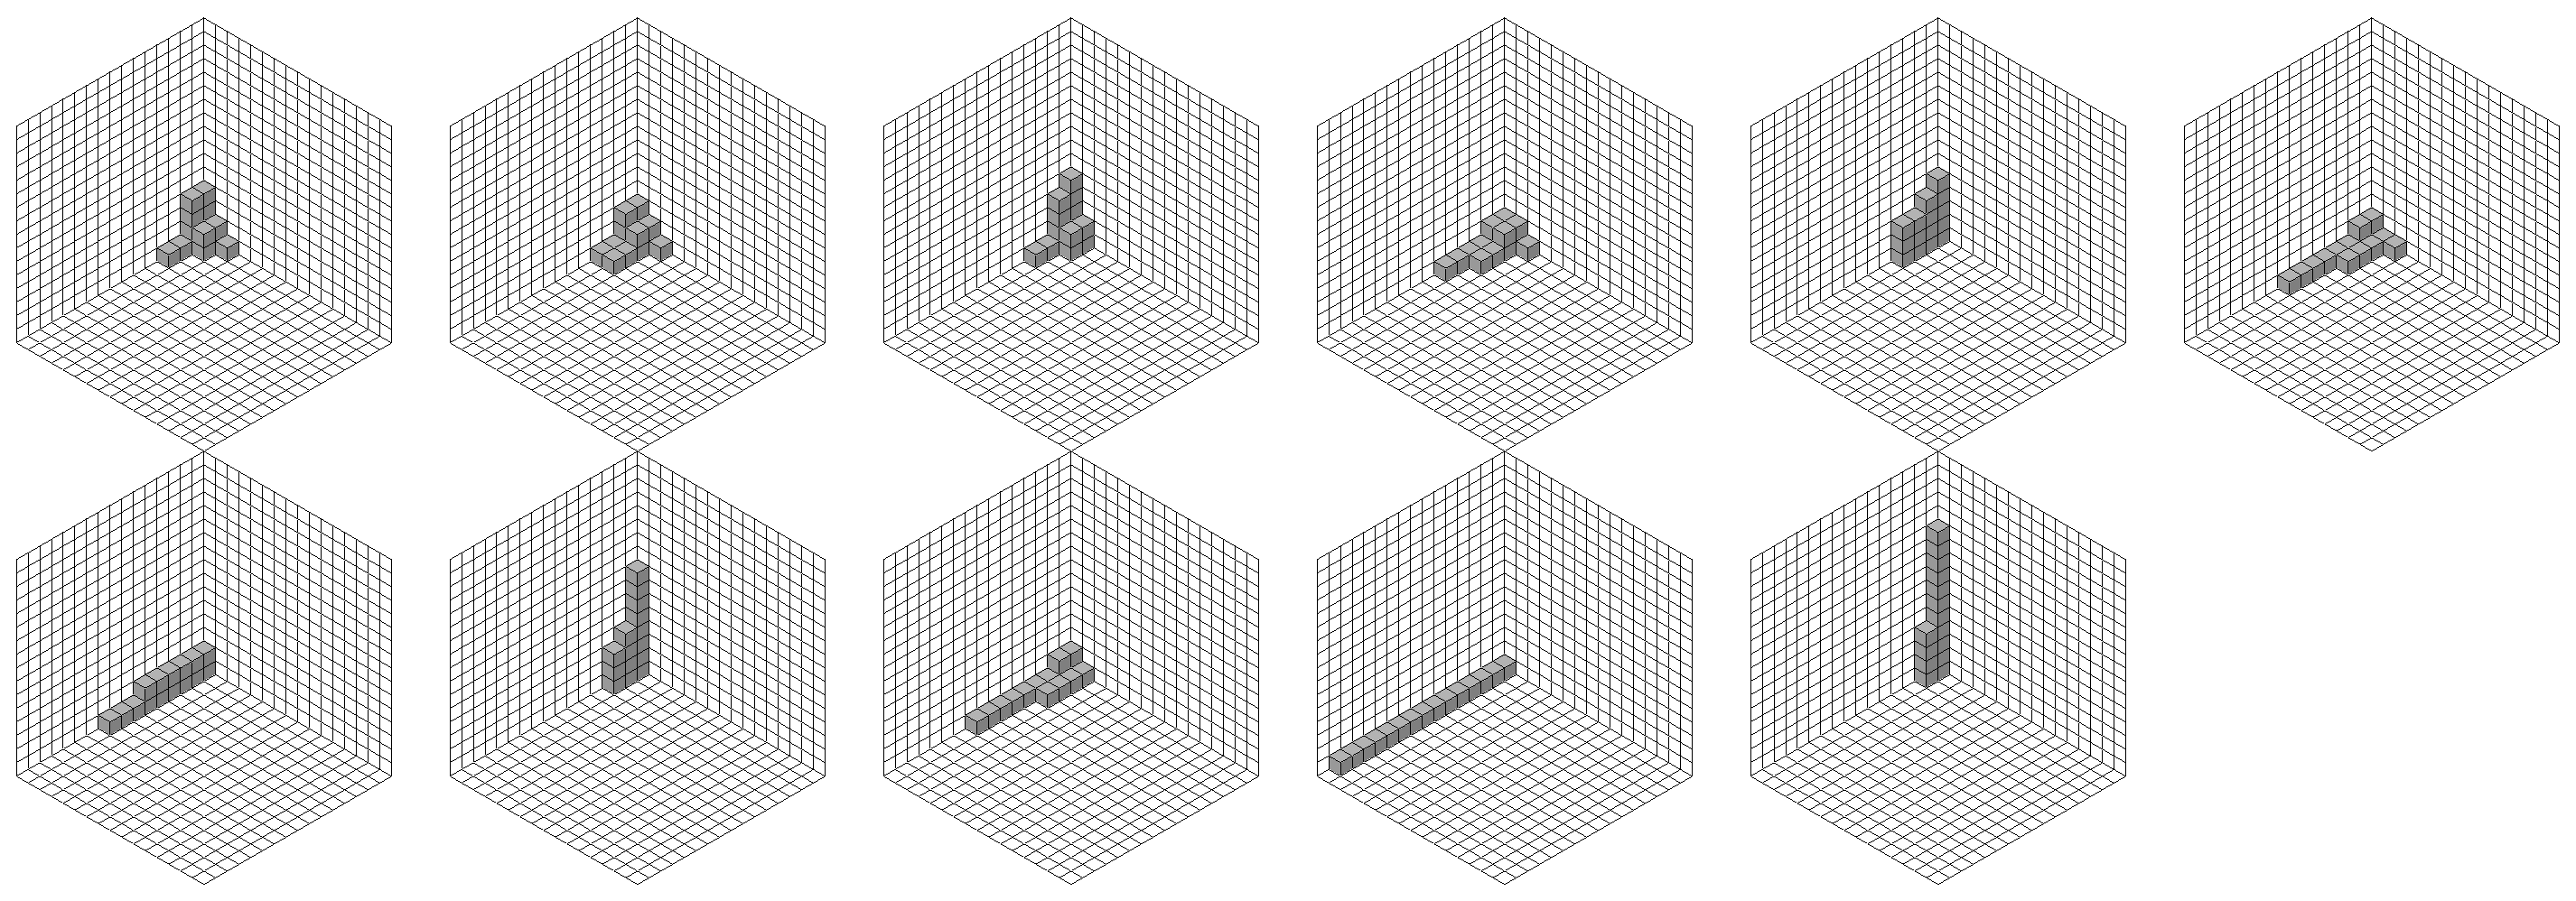
\epsfig{file=staircase.eps,height=4.5cm} 
\end{center}
\caption{Staircase diagrams of the monomial initial ideals in the example - up to symmetry.}
\label{fig:staircase}
\end{figure}
 

In three variables, if we want to draw the Gr\"obner fan - or rather draw the intersection of the $2$-dimensional standard simplex with the Gr\"obner fan we may use the program \texttt{gfan\_render}:
\begin{verbatim}
gfan_bases <myinputfile.txt | gfan_render >myoutputfile.fig
\end{verbatim}
The output is shown in Figure \ref{fig:gfan}.
If there are more than three variables in the polynomial ring this program can still be used but it is more difficult. See Appendix~\ref{applist:_render}.
\begin{figure}
\begin{center}
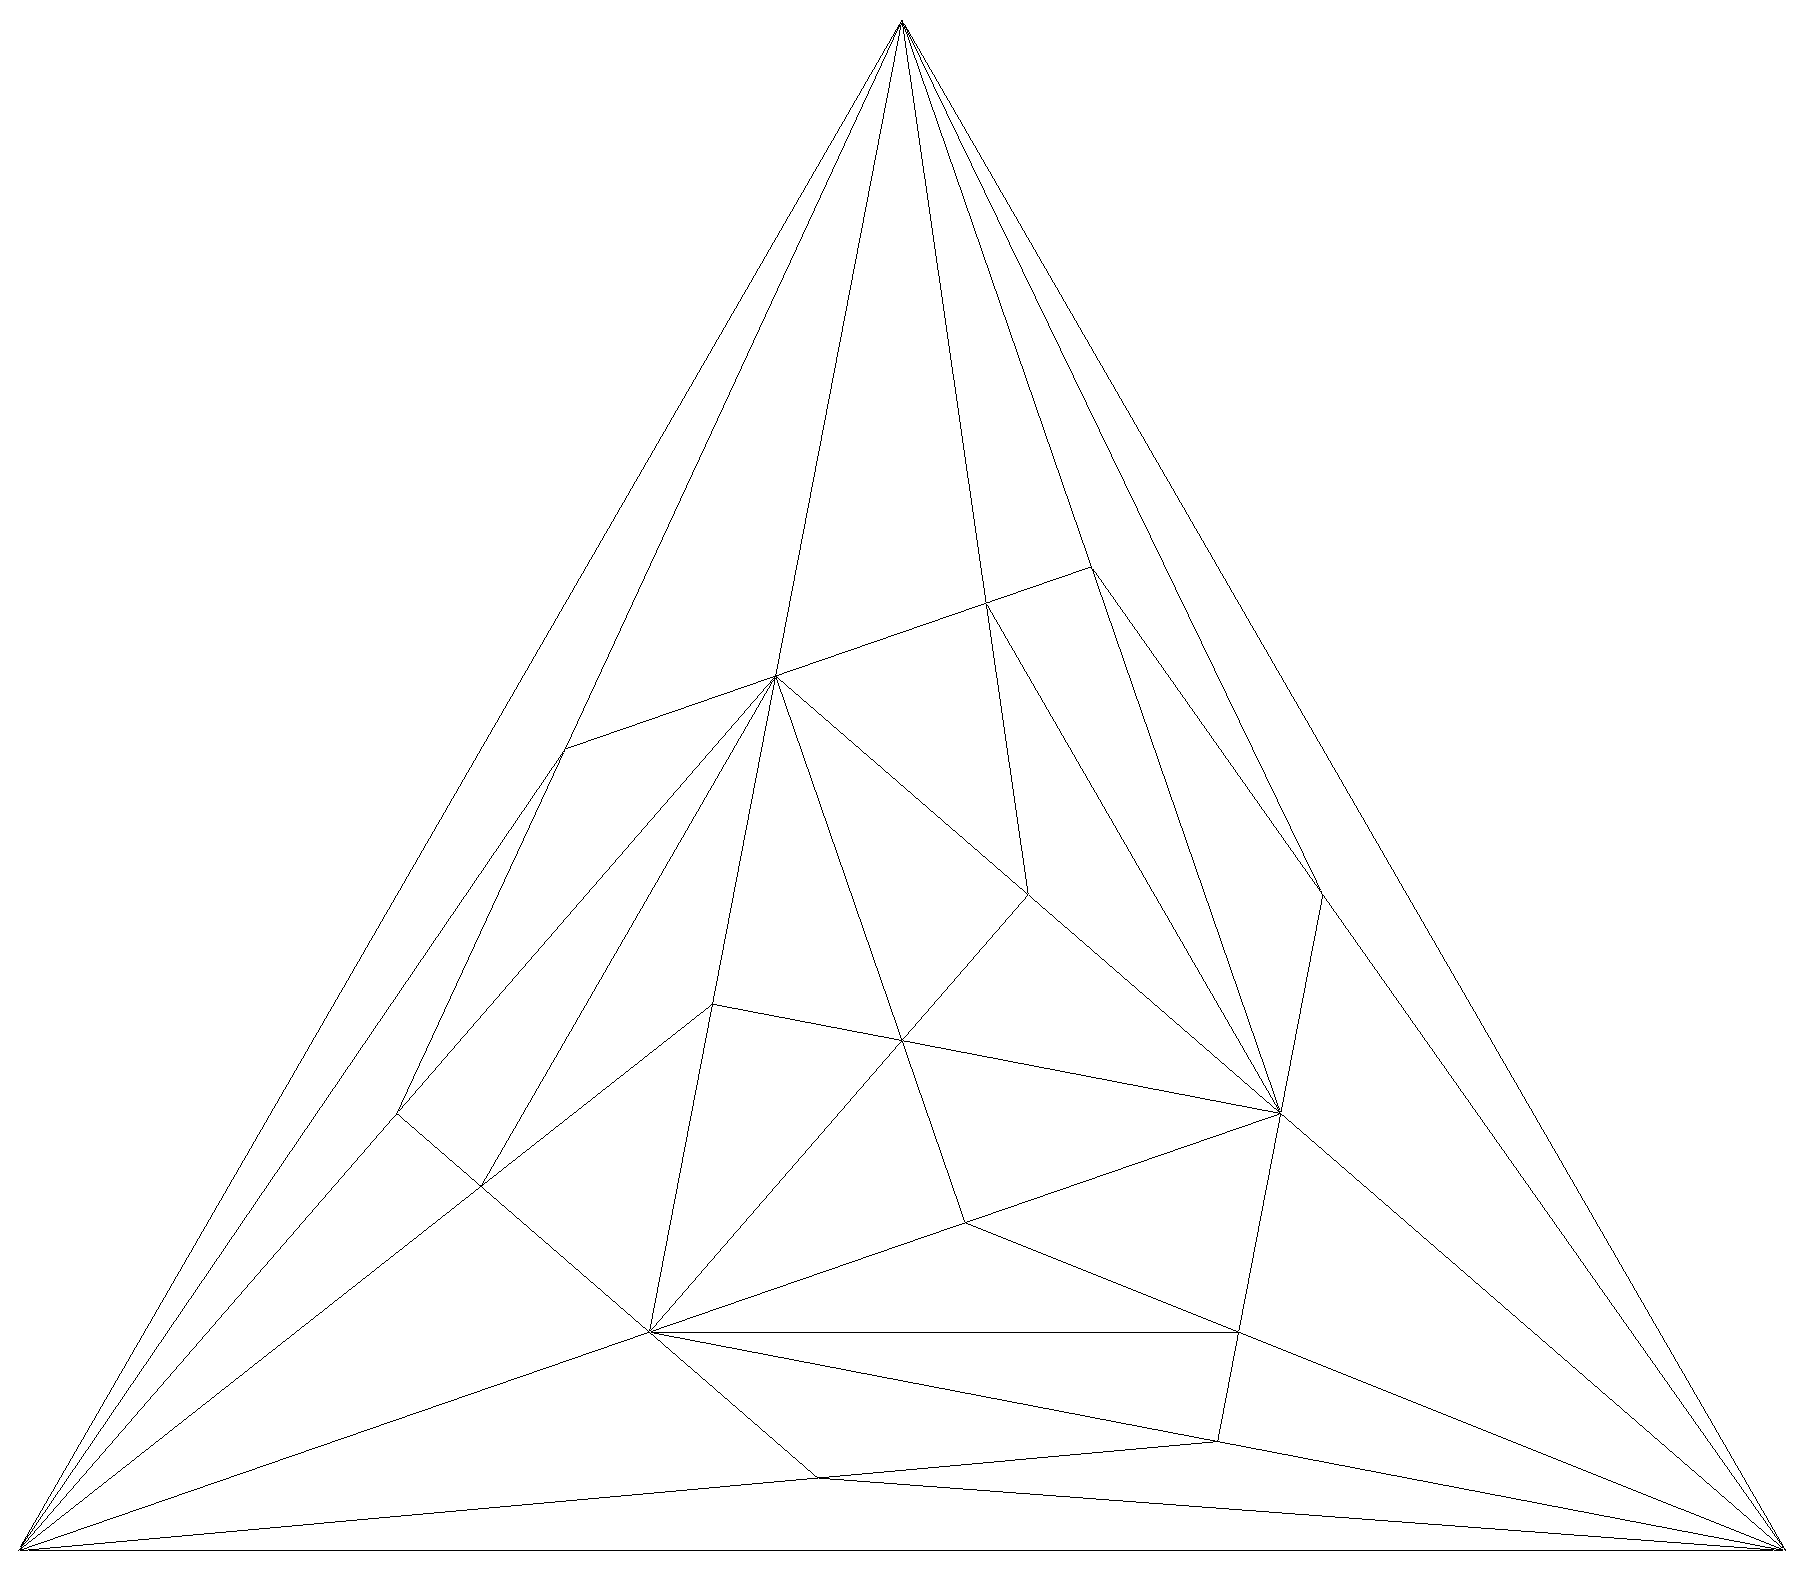
\epsfig{file=gfan.eps,height=5.9cm} 
\end{center}
\caption{The Gr\"obner fan of the ideal intersected with the standard simplex.}
\label{fig:gfan}
\end{figure}

\subsection{Interactive mode}
To study the local structure of the Gr\"obner fan the program \texttt{gfan\_interactive} is useful. It allows the user to walk along an arbitrary path of full dimensional Gr\"obner cones in the Gr\"obner fan of the ideal. At each step the user will specify which facet to walk through. The input must be a marked Gr\"obner basis. The program will minimise and autoreduce if necessary to get the reduced Gr\"obner basis. For example running the program
\begin{verbatim}
gfan_interactive
\end{verbatim}
with input
\begin{verbatim}
Q[a,b,c]
{
c^15-c,
b-c^11,
a-c^9}
\end{verbatim}
will give us a list of facets to walk through. (One way to get a starting Gr\"obner basis is by using the program \texttt{gfan\_buchberger}.) In this case only two flips are possible, since the third wall does not lead to a new Gr\"obner cone. -- The wall is on the boundary of the Gr\"obner region. We may choose any of the two remaining facets by typing in an index (a number) followed by $<$ enter $>$. See Appendix \ref{applist:_interactive} for more options.
%\subsection{Other useful programs}
%We list a few more interesting programs in the package. The remaining programs can be found in Appendix \ref{sec:applist}.
%\subsubsection{Computing a Gr\"obner cone}
%The program \texttt{gfan\_groebnercone} extracts a defining set of half-spaces for a Gr\"obner cone.
%The input is a Gr\"obner basis for the cone. The output is a list of vectors - each specifying a half-space.
%For example we may compute the restricted Gr\"obner cone of the lexicographic basis above by running
%\begin{verbatim}
%gfan_groebnercone --restrict
%\end{verbatim}
%with the reduced Gr\"obner basis as input.
%
%\subsubsection{Computing the facets of a Gr\"obner cone}
%The program \texttt{gfan\_facets} will take a list of vectors - each specifying a half-space whose intersection is a full-dimensional cone and compute a minimal set of defining half-spaces for the cone. Thus, we can compute the inner facet normals of the Gr\"obner cone above by running
%\begin{verbatim}
%gfan_groebnercone --restrict | gfan_facets
%\end{verbatim}
%with the reduced Gr\"obner basis as input.
%
%\subsubsection{Computing a weight vector}
%The program \texttt{gfan\_weightvector} will compute a strictly positive interior point of a Gr\"obner cone given by its reduced Gr\"obner basis. In our example, if we run
%\begin{verbatim}
%gfan_weightvector
%\end{verbatim}
%on the lexicographic basis we (might) get the vector
%\begin{verbatim}
%(21,25,2)
%\end{verbatim}


\subsection{Integers and p-adics}
Gfan handles two settings in which the usual division and Buchberger algorithms do not suffice. These are ideals in $\Z[x_1,\dots,x_n]$ and $\Q[x_1,\dots,x_n]$, where, in the latter setting, the $p$-adic valuation is taken into account when defining initial ideals.

At the moment these two settings are handled by the commands \texttt{gfan\_overintegers} and \texttt{gfan\_padic}. They allow the computation of Gr\"obner bases, initial ideals, Gr\"obner cones (or polyhedra) and Gr\"obner fans (or complexes). In this section we give two examples. Use the \texttt{--help} option to get the full documentation.

\begin{example}
To compute the Gr\"obner fan of \cite[Example~3.9]{sturmfels}, with the ideal considered in the ring $\Z[a,b,c]$ we run the command
\begin{verbatim}
gfan_overintegers --groebnerFan -g --log1
\end{verbatim}
on
\begin{verbatim}
Q[a,b,c]
{a^5+b^3+c^2-1, b^2+a^2+c-1, c^3+a^6+b^5-1}
\end{verbatim}
Since the type-system of Gfan does not understand {\texttt Z[a,b,c]} we need to trick Gfan by specifying the ring $Q[a,b,c]$ when running {\texttt gfan\_overintegers}. From the output we conclude that the ideal has $1659$ reduced Gr\"obner bases over the integers (as opposed to $360$ over a field of characteristic $0$).
\end{example}

\begin{example}
To compute the reduced Gr\"obner basis of $I=\langle x_1+2x_2-3x_3, 3x_2-4x_3+5x_4\rangle\subseteq \Q[x_1,\dots,x_4]$ with respect to the vector $(1,0,0,1)$ (tie-broken lexicographically) and with $\Q$ having the $2$-adic valuation,
we run
\begin{verbatim}
gfan_padic --groebnerBasis -p2
\end{verbatim}
on the input
\begin{verbatim}
Q[x1,x2,x3,x4]
{
x1+2x2-3x3,
3x2-4x3+5x4
}
(1,1,0,0,1)
\end{verbatim}
The first coordinate of the input vector is a $1$, since {\texttt \_padic} requires ``homogenized'' weight vectors. This is Example 2.4.3 in the upcoming book by Maclagan and Sturmfels on tropical geometry. The division algorithm implemented in Gfan used for this computation was proposed by Maclagan. To find all initial ideals, we can use a combination of \texttt{gfan\_padic --groebnerBasis}, \texttt{gfan\_combinerays --section CONES -i filename} and \texttt{gfan\_padic --initialIdeals -m}.

Notice that the Gr\"obner complex of $I$, where valuation is taken into account (see Maclagan-Sturmfels), is not a fan. The output of \texttt{gfan\_groebnerComlex}, however, will be a fan. To get the Gr\"obner complex we need to intersect the fan with the hyperplane $\omega_0=1$.

NOTICE THAT \texttt{\_padic} USES THE MINIMUM CONVENTION AT THE MOMENT - in order to be consistent with Maclagan and Sturmfels.
\end{example}


\subsection{Toric ideals and secondary fans}

Gfan is a replacement of the software CaTS \cite{cats} which computes Gr\"obner fans of toric and lattice ideals.
For convenience a program for computing lattice ideals has been added to Gfan.
To compute the lattice ideal of the lattice generated by $(2,-1,0)$ and $(3,0,-1)$ we run:
\begin{verbatim}
gfan_latticeideal
{(2,-1,0),(3,0,-1)}
\end{verbatim}
Gfan will transform the generators into binomials and compute the
saturation of the ideal they generate by the product of all variables. The computation is independent of the characteristic of the field.

If on the other hand we wish to compute the toric ideal of a \emph{vector configuration} given by the columns of the $1\times 3$-matrix $(1,2,3)$ we run
\begin{verbatim}
gfan_latticeideal -t
{(1,2,3)}
\end{verbatim}
More rows can be added to the matrix if we want.

The choice of the term ``vector configuration'' is intentional and nonstandard. The reason for this will become clear later in this section. In Gfan terminology a \emph{point configuration} is reserved for the collection of points we have before we add a row of ones to construct a projective toric variety. By adding the row of ones the point configuration is turned into a vector configuration.
Notice that scaling a vector of a vector configuration may change its toric ideal.

Computing toric ideals Gfan is not optimal. If one needs to do big examples the software 4ti2 \cite{4ti2} is recommended.

For a toric ideal the radical of a monomial initial ideal is the Stanley-Reisner ideal of a regular triangulation of the point configuration, see \cite{sturmfels}. Hence the toric Groebner fan is a refinement of the \emph{secondary fan}, indexing all regular triangulation of the point configuration.

The secondary fan of the vector configuration $\{(1,0),(1,1),(1,2),(1,3)\}$ can be computed by typing
\begin{verbatim}
gfan_secondaryfan
{(1,0),(1,1),(1,2),(1,3)}
\end{verbatim}
Comparing this to the finer Gr\"obner fan of the corresponding toric ideal which you get by doing
\begin{footnotesize}
\begin{verbatim}
gfan_transposematrix  | gfan_latticeideal -t | gfan_bases | gfan_topolyhedralfan 
{(1,0),(1,1),(1,2),(1,3)}
\end{verbatim}
\end{footnotesize}
you realise that three monomial initial ideals of the toric ideal have the same radical, while four monomial initial ideals pairwise have the same radical.

The secondary fan computation was added for convenience.
%For any
%serious computation with secondary fans you should use
An alternative is to use
TOPCOM \cite{rambau}.  Notice however, that the vector configurations
for gfan\_secondaryfan do not have to be pointed. This means that
all combinatorial types of polytopes with a fixed set of normals can
be easily enumerated. This is not possible with TOPCOM.

\newpage
\section{Doing tropical computations}
\label{sec:tropical}
\emph{This section follows the max convention for tropical
arithmetic. For the non-constant coefficient case tropical varieties are defined as in \cite{lifting} and \cite{thesis}.}
\vspace{0.5cm}

In this section we
explain how to use Gfan to do tropical computations.  For a fixed ideal $I\subseteq
k[x_1,\dots,x_n]$ the set of all faces of all full-dimensional
Gr\"obner cones is a polyhedral complex which we call the Gr\"obner
fan of $I$. For tropical computations the lower dimensional cones of
the complex will be of our interest. In general every Gr\"obner cone
is of the form:
$$C_\omega(I):=\overline{\{\omega'\in\R^n:\init_{\omega'}(I)=\init_\omega(I)\}
}.$$ 

We define the tropical variety $\T(I)$ of an ideal $I$ to be the
the set of all $\omega$ such that $\init_\omega(I)$ does not contain a monomial.
If the ideal $I$ is homogeneous with respect to a positive grading, then the Gr\"obner cones cover all of $\R^n$ and $\T(I)$ is a union of Gr\"obner cones.
Thus for a homogeneous ideal the tropical variety gets the structure of a polyhedral fan which it inherits from the Gr\"obner fan.
%collection of all Gr\"obner cones with monomial-free initial
%ideals.
We therefore also define the tropical variety $\T(I)$ to be the collection of all Gr\"obner cones $C_\omega(I)$ such that $\init_\omega(I)$ is monomial-free.

We start by noticing that for computational purposes it is no restriction to only consider the case of a homogeneous ideal:
\begin{lemma}\cite[Lemma~6.2.5]{thesis}
\label{lem:tropical by homogenisation}
Let $I\subseteq k[x_1,\dots,x_n]$ be an ideal generated by
$f_1,\dots,f_m\in k[x_1,\dots,x_n]$. Let $J=\langle
f_1^h,\dots,f_m^h\rangle\subseteq k[x_0,\dots,x_n]$. Then $\init_\omega(I)$ is monomial-free if and
only if $\init_{(0,\omega)}(J)$ is monomial-free where $\omega\in\R^n$. In particular we have the following identity of sets in $\R^{n+1}$:
$$\{0\}\times\T(I)=\T(J)\cap(\{0\}\times\R^n).$$
\end{lemma}
Here $f^h$ denotes the homogenization of the polynomial $f$.
The homogenization of a list of polynomials can be computed by the program \texttt{gfan\_homogenize}.
Notice that the lemma only requires the generators to be homogenized as a set of polynomials and not in the sense of a polynomial ideal.

The tropical algorithms
implemented in Gfan are explained in \cite{ctv}.
% The reference also
%contains definitions and theorems needed for understanding this
%section of the manual.
Notice that Gfan follows the usual conventions
for signs of weight vectors defining initial forms while \cite{ctv}
uses opposite signs. This means that \name is compatible with the max-plus convention whereas \cite{ctv} is compatible with the min-plus convention.

\subsection{Tropical variety by brute force}
The command \texttt{gfan\_tropicalbruteforce} will compute all
Gr\"obner cones of a homogeneous ideal and for each check if its initial ideal
contains a monomial. The output is the tropical variety of the
ideal. Since the tropical variety is usually much smaller than the
Gr\"obner fan this is a rather slow method for computing the tropical
variety. The line
\begin{verbatim}
gfan_buchberger | gfan_tropicalbruteforce
\end{verbatim}
run on the input
\begin{verbatim}
Q[a,b,c,d,e,f,g,h,i,j]
{
bf-ah-ce,
bg-ai-de,
cg-aj-df,
ci-bj-dh,
fi-ej-gh
}
\end{verbatim}
produces a tropical variety of the input ideal in a few minutes as a
polyhedral fan, see Section~\ref{format:fan}. We use
\texttt{gfan\_buchberger} since \texttt{gfan\_tropicalbruteforce}
requires its input to be a marked reduced Gr\"obner basis.
\begin{remark}
Notice that if $k'\supseteq k$ is a field extension and $I\subseteq
k[x_1,\dots,x_n]$ an ideal then $\T(I)=\T(\langle
I\rangle_{k'[x_1,\dots,x_n]})$ as a polyhedral fan. This identity
follows since both objects can be computed by Gr\"obner basis methods
and Gr\"obner bases are independent of such field extensions. The same argument of course also applies to the Gr\"obner fans of the two ideals.
\end{remark}
\subsection{Traversing tropical varieties of prime ideals}
Let $I\subseteq \CC[x_1,\dots,x_n]$ be a homogeneous monomial-free
prime ideal of dimension $d$. By the Bieri Groves Theorem \cite{bg}
the tropical variety of $I$ is a pure $d$-dimensional polyhedral
fan. It is connected in codimension one (\cite[Theorem~14]{ctv}) and can be
traversed by Gfan. Let $\omega$ be a relative interior point of a
$d$-dimensional Gr\"obner cone in the tropical variety of $I$. Fix
some term order $\prec$. Gfan represents $C_\omega(I)$ by the pair of
marked reduced Gr\"obner bases
$(\G_{\prec_\omega}(\init_\omega(I)),\G_{\prec_\omega}(I))$.  To
compute the tropical variety of an ideal we must begin by finding a
starting $d$-dimensional Gr\"obner cone. For this
\texttt{gfan\_tropicalstartingcone} is used. This programs guesses a
starting cone by heuristic methods. The guessing might fail. In that
case the program will terminate with an error message.  After having
computed a starting cone we use the program
\texttt{gfan\_tropicaltraverse} to traverse the tropical variety.
%There are several options for the output. In general the choice of output we request can have a huge influence on the running time for the program.
We illustrate the procedure with an example.
\begin{remark}
Gfan does its computations over $\Q$ and thus the input should be an
ideal generated by polynomials in $\Q[x_1,\dots,x_n]$. The assumption
that $I$ is an ideal in $\CC[x_1,\dots,x_n]$ is needed since by
``prime ideal'' in the above we mean ``prime ideal in the polynomial
ring over the algebraically closed field $\CC$''. If $I$ is a prime ideal in
$\Q[x_1,\dots,x_n]$ we do not know that its tropical variety is connected.
 In
Section~\ref{sec:non-constant} we address the problem of specifying non-rational
coefficients.
\end{remark}
\begin{example}
Let $I\subseteq\Q[a,\dots,o]$ be the ideal generated by the relations
on the 2 by 2 minors of a 2 by 6 generic matrix.  In $\CC[x_1,\dots,x_n]$ the
ideal $I$ generates a prime ideal.  To get a starting cone for the
traversal of $\T(I)$ we run the command
\begin{verbatim}
gfan_tropicalstartingcone
\end{verbatim}
on the input
\begin{verbatim}
Q[a,b,c,d,e,f,g,h,i,j,k,l,m,n,o]
{
bg-aj-cf,  bh-ak-df,  bi-al-ef,  ck-bm-dj,  ch-am-dg,
cl-ej-bn,  ci-eg-an,  dn-co-em,  dl-bo-ek,  di-ao-eh,
gk-fm-jh,  gl-fn-ij,  hl-fo-ik,  kn-jo-lm,  hn-im-go
}
\end{verbatim}
and get a pair of marked reduced Gr\"obner bases
\begin{verbatim}
Q[a,b,c,d,e,f,g,h,i,j,k,l,m,n,o]
{
l*m+j*o,  i*m+g*o,  i*k-h*l,  i*j-g*l,  h*j-g*k,
e*m+c*o,  e*k+b*o,  e*j-c*l,  e*h+a*o,  e*g-c*i,
c*k-b*m,  c*h-a*m,  b*i-a*l,  b*h-a*k,  b*g-a*j}
{
l*m-k*n+j*o, i*m-h*n+g*o, i*k-h*l+f*o, i*j-g*l+f*n, h*j-g*k+f*m,
e*m-d*n+c*o, e*k-d*l+b*o, e*j-c*l+b*n, e*h-d*i+a*o, e*g-c*i+a*n,
c*k-d*j-b*m, c*h-d*g-a*m, b*i-e*f-a*l, b*h-d*f-a*k, b*g-c*f-a*j}
\end{verbatim}
This takes a minute or so. We store the output in the file \texttt{grassmann2\_6.cone} for later use. Since $I$ has many symmetries we add the following lines describing the symmetry group to the end of the file:
\begin{verbatim}
{
(0,8,7,6,5,4,3,2,1,14,13,11,12,10,9),
(5,6,7,8,0,9,10,11,1,12,13,2,14,3,4)
}
\end{verbatim}
We are ready to traverse $\T(I)$.
% We start by running the program with the simplest possible output and using symmetries:
We run the following command
\begin{verbatim}
gfan_tropicaltraverse --symmetry <grassmann2_6.cone
\end{verbatim}
The computation takes a few (two - three) minutes. The output looks like this:
\begin{verbatim}
_application PolyhedralFan
_version 2.2
_type PolyhedralFan

AMBIENT_DIM
15

DIM
9

LINEALITY_DIM
6

RAYS
0 0 -1 0 0 0 0 0 0 0 0 0 0 0 0	# 0
0 0 0 0 0 0 0 -1 0 0 0 0 0 0 0	# 1
0 0 0 0 0 0 0 0 0 0 0 -1 0 0 0	# 2
0 0 0 -1 0 0 0 0 0 0 0 0 0 0 0	# 3
0 0 0 0 0 0 -1 0 0 0 0 0 0 0 0	# 4
0 -1 0 0 0 0 0 0 0 0 0 0 0 0 0	# 5
0 0 0 0 0 0 0 0 -1 0 0 0 0 0 0	# 6
0 0 0 0 0 0 0 0 0 0 -1 0 0 0 0	# 7
0 0 0 0 0 0 0 0 0 0 0 0 0 -1 0	# 8
0 0 0 0 0 -1 0 0 0 0 0 0 0 0 0	# 9
0 0 0 0 -1 0 0 0 0 0 0 0 0 0 0	# 10
0 0 0 0 0 0 0 0 0 0 0 0 0 0 -1	# 11
0 0 0 0 0 0 0 0 0 -1 0 0 0 0 0	# 12
-1 0 0 0 0 0 0 0 0 0 0 0 0 0 0	# 13
0 0 0 0 0 0 0 0 0 0 0 0 -1 0 0	# 14
0 0 0 -1 -1 -1 -1 0 0 -1 0 0 0 0 -1	# 15
-1 -1 0 0 0 -1 0 0 0 0 0 0 -1 -1 -1	# 16
-1 0 0 0 -1 0 0 0 -1 -1 -1 0 -1 0 0	# 17
1 1 0 0 0 1 2 2 0 2 2 0 1 1 1	# 18
1 0 2 2 1 0 0 0 1 1 1 0 1 2 2	# 19
0 0 0 1 1 1 1 0 0 1 2 2 2 2 1	# 20
1 1 0 2 2 1 0 2 2 0 0 0 1 1 1	# 21
1 2 2 0 1 2 2 0 1 1 1 0 1 0 0	# 22
2 2 0 1 1 1 1 0 2 1 0 2 0 0 1	# 23
0 -1 0 -1 0 0 -1 0 -1 0 -1 0 0 -1 0	# 24

N_RAYS
25

LINEALITY_SPACE
0 0 0 0 0 1 1 1 1 1 1 1 1 1 1
0 0 0 0 1 0 0 0 1 0 0 1 0 1 1
0 0 0 1 0 0 0 1 0 0 1 0 1 0 1
0 0 1 0 0 0 1 0 0 1 0 0 1 1 0
0 1 0 0 0 0 -1 -1 -1 0 0 0 -1 -1 -1
1 0 0 0 0 0 0 0 0 -1 -1 -1 -1 -1 -1

ORTH_LINEALITY_SPACE
0 0 0 0 0 0 0 0 0 0 1 -1 -1 1 0
0 0 0 0 0 0 0 0 0 1 0 -1 -1 0 1
0 0 0 0 0 0 0 1 -1 0 0 0 -1 1 0
0 0 0 0 0 0 1 0 -1 0 0 0 -1 0 1
0 0 0 0 0 1 0 0 -1 0 0 -1 -1 1 1
0 0 0 1 -1 0 0 0 0 0 0 0 -1 1 0
0 0 1 0 -1 0 0 0 0 0 0 0 -1 0 1
0 1 0 0 -1 0 0 0 0 0 0 -1 -1 1 1
1 0 0 0 -1 0 0 0 -1 0 0 0 -1 1 1

F_VECTOR
1 25 105 105
\end{verbatim}
After this follows a list of cones and maximal cones.
Every maximal cone has an associated multiplicity which is also listed.

The output says that the tropical variety has dimension $9$. Modulo the
$6$-dimensional homogeneity space this is reduced to a $3$-dimensional complex in
$\R^9$ and thus we may think of the tropical variety as a
$2$-dimensional polyhedral complex on the $8$-sphere in $\R^9$. This
complex is simplicial and has $105$ maximal cones.


The extreme rays (modulo the homogeneity space) are labeled
$0,\dots,24$. In the cone lists the cones are grouped together
according to dimension and orbit with respect to the specified
symmetries. See Section~\ref{sec:format fan} for more information on how to read the
polyhedral fan format.
\end{example}

%If we look carefully in the debug output from the program we
%will also see that these $105$ cones come in $17$ orbits.  If we
%wanted to know more about the traversed cones we could use the option
%\texttt{--largedimensional}. This will list the $d$-dimensional and
%$(d-1)$-dimensional cones of the fan. In our example one of the
%$d$-dimensional cones is listed like this: (In this manual lines have
%been concatenated to avoid wasting paper)

While traversing the variety the program
\texttt{gfan\_tropicaltraverse} only computes $d$ and
$(d-1)$-dimensional cones. The other cones are extracted after
traversing. Also the symmetries are expanded. Sometimes extracting all
cones is time consuming and one is only interested in the high
dimensional cones up to symmetry. These can be output using the option
\texttt{--noincidence}. In that case the output would be a list of
orbits for maximal cones and a list of orbits for codimension one
cones. It is also listed how these cones are connected taking symmetry
into account. In general that format is rather difficult to read.


A final remark about \texttt{gfan\_tropicaltraverse} is that the
polyhedral structure of the complex comes from the Gr\"obner fan. For
some ideals it is possible to find polyhedral fans covering the
tropical variety with fewer cones.


\subsection{Intersecting tropical hypersurfaces}
The tropical variety of a principal ideal is called a \emph{tropical
hypersurface}. A \emph{tropical prevariety} is a finite intersection of
tropical hypersurfaces or, to be precise, the intersection of the
support set of these hypersurfaces. In Gfan the intersection is
represented by the \emph{common refinement} of the tropical
hypersurfaces. The program \texttt{gfan\_tropicalintersection} can
compute such intersections.
\begin{example}
To compute the intersection of the tropical hypersurfaces $\T(\langle a+b+c+1\rangle)$ and $\T(\langle a+b+2c\rangle)$ we run
\begin{verbatim}
gfan_tropicalintersection
\end{verbatim} 
on
\begin{verbatim}
Q[a,b,c]
{a+b+c+1,a+b+2c}
\end{verbatim}
The output is a polyhedral fan whose support is the intersection. The
balancing condition for this fan is not satisfied which implies that it
is not a tropical variety.
%list of cones whose union is the tropical prevariety.  Notice, as a polyhedral complex, some cones might be missing from the list but all maximal cones are present. The program also gives a list with a relative interior point for each cone. 

%If we use the option \texttt{--incidence} we will get more information about the combinatorial structure of the intersection as a polyhedral complex. We should note that this option only investigates the maximal dimensional complex.

%An interesting question is if the intersection equals the tropical variety of the ideal generated by the input polynomials. A necessary condition for this to be true is that all the computed relative interior points pick out monomial-free initial ideal. This can be checked with the option \texttt{-t}. In our example the prevariety is not equal to the tropical variety and the program will find a vector that proves this.
\end{example}

\subsection{Computing tropical bases of curves}
In Gfan an ideal $I$ is said to define a \emph{tropical curve} if
$k[\x_1,\dots,x_n]/I$ has Krull dimension equal to or one larger than the
dimension of the homogeneity space of $I$.  A \emph{tropical basis} of $I$ is
a finite generating set for the ideal such that the tropical variety
defined by $I$ (as a set) is the intersection of the tropical
hypersurfaces of the generators. A tropical basis always exists \cite{ctv}.  The
program \textup{gfan\_tropicalbasis} computes a tropical basis for an
ideal defining a tropical curve.
\begin{example}
Again we consider the ideal $\langle a+b+c+1,a+b+2c\rangle$. We notice that this ideal defines a curve since the Krull dimension is $1$ and the dimension of the homogeneity space is $0$. In the example above we saw that the listed set is not a tropical basis. We run
\begin{verbatim}
gfan_tropicalbasis -h
\end{verbatim}
on
\begin{verbatim}
Q[a,b,c]
{a+b+c+1,a+b+2c}
\end{verbatim}
to get some tropical basis
\begin{verbatim}
Q[a,b,c]
{
-1+c,
2+b+a}
\end{verbatim}
We needed the option \texttt{-h} here since the ideal was not homogeneous. If we run \texttt{gfan\_tropicalintersection} on the output we see that the tropical variety consists of three rays and the origin.
\end{example}


\subsection{Tropical intersection theory}
Gfan contains a few experimental programs for doing computations in
tropical intersection theory. In \cite[Definition 3.4]{allermannRau}
the tropical Weil divisor of a tropical rational function on a
(tropical) $k$-cycle in $\R^n$ is defined. This divisor can be
computed in Gfan. However, Gfan and \cite{allermannRau} do not agree
on the basic definitions in tropical geometry. For example the
definition of a fan is different. Here we will adjust the necessary
definitions to the Gfan conventions. A tropical $k$-cycle will be a
pure (rational) polyhedral fan $F$ of dimension $k$ in $\R^n$ with
weights which is balanced in the following sense: To every
$k$-dimensional facet $C$ we assign a weight (or multiplicity)
$m_C\in\Z$. The vector space $\R^n$ comes with its standard lattice
$\Z^n$. For a $k-1$-dimensional ridge $R\in F$ and a facet $C$ in its
star\footnote{the smallest polyhedral subcomplex of $F$ containing all
faces of $F$ containing $R$.} in $F$ corresponding to a cone $L$ in
the link\footnote{take an $\epsilon$-ball around a relative interior
$\omega\in R$ and intersect it with $F$. Translating the ball to the
origin and scaling the intersection to infinity we get the link of $R$
in $F$.} of $R$ in $F$, the semi-group
$L\cap\Z^n/\textup{span}_{\R}(R)\cap\Z^n\subseteq
\Z^n/\textup{span}_{\R}(R)\cap\Z^n$ is isomorphic to $\N$. Define
$u_{C/R}\in \Z^n/\textup{span}(R)\cap\Z^n$ as the element identified
with $1\in\N$. The balancing condition at $R$ is that
$$\sum_{C\in F:R\subset C} m_Cu_{C/R}=0.$$
For a (weighted) fan to be a tropical cycle this must hold at every ridge $R$.

It remains to define what a tropical rational function is. Take a
polyhedral fan $F'$ and associate to each of its maximal cones a
linear form. When evaluating a point $x$ in the support of $F'$ simply
evaluate the linear form of cone containing $x$. If this gives a
well-defined function we call this function a tropical rational
function.  When computing Weil divisors we will require that the supports satisfy
$\textup{supp}(F)\subseteq \textup{supp}(F')$.  There will be no further restriction
on the polyhedral structure.

For a definition of the Weil divisor itself we refer
to \cite[Definition 3.4]{allermannRau}. Here we just mention that it
again is a cycle of dimension one lower.

To demonstrate the Gfan features we recompute \cite[Example 3.10]{allermannRau}.
An easy way to generate the $k$-cycle of that example is to compute it as a hypersurface. Since the paper is using min and Gfan is using max we need to change the polynomial from the paper such that the Newton polytope is flipped:
\begin{verbatim}
gfan_tropicalhypersurface > tmpfile1.poly
Q[x_1,x_2,x_3]
{x_2x_3+x_1x_3+x_1x_2+x_1x_2x_3}
\end{verbatim}
The weights/multiplicities are stored in the MULTIPLICITIES section of the Polymake file.

It is harder specifying the rational function. We make the following file and call in \texttt{func.poly}.
\begin{footnotesize}
\begin{verbatim}
_application PolyhedralFan
_version 2.2
_type PolyhedralFan

AMBIENT_DIM
3

DIM
2

LINEALITY_DIM
0

RAYS
1 0 0	# 0
0 1 0	# 1
0 0 1	# 2
-1 -1 -1	# 3
1 1 0	# 4
-1 -1 0	# 5

N_RAYS
6

LINEALITY_SPACE

ORTH_LINEALITY_SPACE
1 0 0
0 1 0
0 0 1

MAXIMAL_CONES
{3 5}	# Dimension 2
{5 2}
{0 2}
{1 2}
{1 3}
{0 3}
{1 4}
{0 4}

MULTIPLICITIES
1
1
1
1
1
1
1
1

RAY_VALUES
0
0
0
1
-1
0

LINEALITY_VALUES
\end{verbatim}
\end{footnotesize}
Instead of specifying the linear function on each maximal cone we have
to specify its values on each of the rays in the fan and each of the
generators of the lineality space. Then Gfan will automatically
interpolate the function. Since the lineality space of the fan is
empty we leave the LINEALITY\_VALUES section empty.

We now compute the Weil divisor:
\begin{footnotesize}
\begin{verbatim}
gfan_tropicalweildivisor -i1 tmpfile1.poly -i2 func.poly >tmpfile2.poly
\end{verbatim}
\end{footnotesize}
...and compute the Weil divisor again as in \cite{allermannRau}...
\begin{footnotesize}
\begin{verbatim}
gfan_tropicalweildivisor -i1 tmpfile2.poly -i2 func.poly >tmpfile3.poly
\end{verbatim}
\end{footnotesize}
We get a fan with the origin being the only cone. It has multiplicity $-1$:
\begin{verbatim}
MULTIPLICITIES
-1      # Dimension 0
\end{verbatim}

There is another useful command for computing polyhedral fans for
rational functions. The command \texttt{gfan\_tropicalfunction} takes a
polynomial and turns it into a fan representing its tropicalization
which is a tropical rational function.

\subsection{Non-constant coefficients}
\label{sec:non-constant}
In tropical geometry it is common to take the valuation of
$\CC\{\{t\}\}$ into account when defining the tropical variety of
an ideal in $\CC\{\{t\}\}[x_1,\dots,x_n]$.  Here $\CC\{\{t\}\}$ denotes the field of
Puiseux series. The valuation $\textup{val}(p)$ of a non-zero Puiseux
series $p$ is the degree of its lowest order term.


\begin{definition}
For $\omega\in\R^n$ the \emph{t-$\omega$-degree}\index{t-$\omega$-degree} of a term $ct^ax^v$
with $c\in\CC^*$, $a\in \Q$ and $v\in\Z^n$ is defined as
$-\val(ct^a)+\omega\cdot v=-a+\omega\cdot v$.  The \emph{t-initial
form}\index{t-initial form} $\tinit_\omega(f)\in\CC[x_1,\dots,x_n]$ of a polynomial
$f\in\puiseux[x_1,\dots,x_n]$ is the sum of all terms in $f$ of maximal
t-$\omega$-weight but with $1$ substituted for $t$.
\end{definition}
\begin{remark}
Notice that since $t$ has t-$\omega$-degree $-1$, the maximal
t-$\omega$-weight \emph{is} attained by a term if the polynomial is
non-zero. Furthermore, only a finite number of terms attain the
maximum. Therefore, it makes sense to substitute $t=1$ and consider
the finite sum of terms as a polynomial in $\CC[x_1,\dots,x_n]$.
\end{remark}
\begin{example}
Consider $f=(1+t)+t^2x+tx^2\in\puiseux[x_1,\dots,x_n]$. Let $\omega=({1\over
2})\in\R^1$. Then $\tinit_\omega(f)=1+x^2$. For any
other choice of $\omega$ the t-initial form is a monomial.
\end{example}
\begin{definition}
Let $I\subseteq \puiseux[x_1,\dots,x_n]$ and $\omega\in\R^n$. The \emph{t-initial ideal}\index{t-initial ideal} of $I$ with respect to $\omega$ is defined as:
$$\tinit_\omega(I):=\langle \tinit_\omega(f):f\in I\rangle\subseteq\CC[x_1,\dots,x_n].$$
\end{definition}

\begin{definition}
\label{def:tropvar}
Let $I\subseteq \puiseux[x_1,\dots,x_n]$ be an ideal. The \emph{tropical variety} of $I$ is the set
$$\T'(I):=\{\omega\in\R^n:\tinit_\omega(I) \textup{ is monomial-free}\}.$$
%Here monomial-free\index{monomial-free} means that the ideal does not contain a monomial.
\end{definition}
We use the notation $\T'(I)$ to avoid contradicting our original definition
of the tropical variety of an ideal in the polynomial ring over a
field.
%An important theorem says that the tropical variety of $I$ is also the
%negative of the closure of the image of $V(I)\subseteq \CC\{\{t\}\}^*$
%under the coordinatewise valuation.


\begin{proposition} \cite[Proposition~7.3]{lifting}
\label{prop:computing tinit}
Let $I\subseteq \CC[t,x_1,\dots,x_n]$ be an ideal, $J=\langle I\rangle_{\puiseux[x_1,\dots,x_n]}$ and $\omega\in\R^n$. Then $\textup{t-in}_\omega(I)=\textup{t-in}_\omega(J)$.
\end{proposition}

\begin{remark}
\label{rem:computing tinit}
For $f\in\CC[t,x_1,\dots,x_n]$ we have
$\tinit_\omega(f)=(\init_{(-1,\omega)}(f))|_{t=1}$. Consequently, for
$I\subseteq\CC[t,x_1,\dots,x_n]$ we have
$\tinit_\omega(I)=(\init_{(-1,\omega)}(I))|_{t=1}$. In order to
decide if $\tinit_\omega(I)$ contains a monomial we may simply decide if the initial ideal
$\init_{(-1,\omega)}(I)$ contains a monomial.
 As a corollary we get
$$\T(I)\cap(\{-1\}\times\R^n)=\{-1\}\times\T'(J).$$

In fact this gives a method for computing the tropical variety as a set of any
ideal $J\subseteq\CC\{\{t\}\}[x_1,\dots,x_n]$ generated by elements
in the polynomial ring over the field of rational functions
$\Q(t)[x_1,\dots,x_n]$ in Gfan by clearing denominators and
intersecting the result with the $t=-1$ plane.  (We remind the reader
that Lemma~\ref{lem:tropical by homogenisation} shows that for
computational purposes it is no restriction if $I$ is not
homogeneous.)
\end{remark}

Intersecting the tropical variety with the $t=-1$ plane can with some difficulty be done by
hand. If the tropical (pre)-variety has been computed with
\texttt{gfan\_tropicalintersection} then it is also possible to let Gfan do
the intersection. What Gfan does is to compute the common refinement
of the fan with the fan consisting of the halfspace $t\leq 0$ and its
proper face. Of course this does not remove the cones in the $t=0$
plane, but they are easily removed by hand. We illustrate the
procedure by an example.

\begin{example}
\label{ex:nonconstant}
Exercise 2 in Chapter 9 of \cite{sturmfelssolving} asks us to draw the variety
defined by the \emph{tropical} polynomial
$f=1x^2+2xy+1y^2+3x+3y+1$. If we tropically divide this polynomial by $3$ we get $f':=f/3=-2x^2-1xy-2y^2+0x+0y+-2$ which defines the same tropical variety. This variety equals the variety defined by
the polynomial $g=t^2x^2+txy+t^2y^2+x+y+t^2\in\CC\{\{t\}\}[x,y]$. Notice that $f'$ is the tropicalisation of $g$.

According to Remark~\ref{rem:computing tinit} above the we may compute $\T'(\langle g\rangle)$ by computing
the variety of $\langle t^2x^2+txy+t^2y^2+x+y+t^2\rangle\subseteq \CC[t,x,y]$ and intersecting it with the hyperplane $t=-1$.
Running
\begin{verbatim}
gfan_tropicalintersection --tplane
\end{verbatim}
on
\begin{verbatim}
Q[t,x,y]
{t^2x^2+txy+t^2y^2+x+y+t^2}
\end{verbatim}
we get
\begin{verbatim}
RAYS
0 -1 0	# 0
-1 2 1	# 1
0 1 1	# 2
-1 1 1	# 3
-1 -2 -2	# 4
0 0 -1	# 5
-1 1 2	# 6

MAXIMAL_CONES
{3 4}	# Dimension 2
{2 6}
{1 3}
{1 2}
{3 6}
{4 5}
{0 4}
{0 6}
{1 5}
\end{verbatim}
among other information. We can now draw the two-dimensional picture
asked for in the exercise.  The rays with non-zero first coordinate
become points in the picture. (If the first coordinate is not $-1$ scaling
is required to get the rational $x,y$-coordinates.) The rays with zero
first coordinate become directions. The maximal cones show how to
connect the rays; see Figure~\ref{fig:nonconstant}. Notice that some
of the connections could have been ``at infinity''.
\begin{figure}
\begin{center}

\epsfig{file=nonconst.eps,height=5.5cm} 
\end{center}
\caption{The tropical variety defined by the tropical polynomial in Example~\ref{ex:nonconstant}.}
\label{fig:nonconstant}
\end{figure}

\end{example}

\subsubsection{Algebraic field extensions of $\Q$}
Ignoring time, memory usage and overflows Gfan can compute the tropical variety $\T'(I)$ of any ideal $I\subseteq \puiseux[x_1,\dots,x_n]$ generated by elements of $\overline{\Q}(t)[x_1,\dots,x_n]$. This is a consequence of the following lemma:
\begin{lemma}\cite[Lemma~3.12]{lifting}
\label{lem:fieldextension}
Let $k$ be a field and $M=\langle m\rangle\subseteq k[a]$ a maximal ideal where $m$ is not a monomial. Let 
$I\subseteq (k[a]/M)[x_1,\dots,x_n]$ be an ideal. For $\omega\in\R^n$ we
have
$$\init_\omega(I) \textup{ contains a monomial} \Longleftrightarrow \init_{(0,\omega)}(\varphi^{-1}(I)) \textup{ contains a monomial}$$ 
where $\varphi:k[a,x_1,\dots,x_n]\rightarrow (k[a]/M)[x_1,\dots,x_n]$ is the homomorphism taking elements to their cosets.
\end{lemma}


\newpage
\appendix
\section{Data formats}
\label{sec:dataformats}

In this section we describe how polynomials, lists, marked Gr\"obner
bases etc. are represented as ASCII character strings. These strings
will be input to the programs by typing or by redirecting the standard
input and be output by the program on the standard output which may be
the screen, a pipe or a file. Usually files are used for input. For
example,
\begin{verbatim}
gfan_bases < inputfile.txt > outputfile.txt
\end{verbatim}
will read its input from {\tt inputfile.txt} and write its output to
{\tt outputfile.txt}. The following is an example of how to use pipes
for computing a universal Gr\"obner basis of the input:
\begin{verbatim}
gfan_bases < inputfile.txt | gfan_polynomialsetunion > outputfile.txt
\end{verbatim}
In general spaces and newlines in the input are ignored, but for the
polyhedral formats described in Section~\ref{sec:format fan} and
Section~\ref{sec:format cone} the rules are different.

\subsection{Fields}
Two kinds of fields are supported:
\begin{itemize}
\item The field $\Q$ of rationals which is represented by the string ``\texttt{Q}''.
\item Fields of the form $\Z/p\Z$ where $p$ is a prime number. These
fields are represented by text strings ``\texttt{Z/pZ}'' where \texttt{p}  is the
prime number. For example ``\texttt{Z/3Z}'' or ``\texttt{Z/17Z}''. In Gfan the
prime number $p$ must be less than $32749$.
\end{itemize}
\subsection{Variables}
A variable is denoted by its name which is an string of
characters. The exact rules for which names are allowed have not been
decided on in this version of Gfan and therefore Gfan accepts most
names. However, white spaces, commas and ``\texttt{]}'' are not allowed
as characters in the name. Furthermore one should not choose variable
names such that one name is a starting substring of an other -- don't
choose names such as ``\texttt{x1}'' and ``\texttt{x}''
in the same polynomial ring.
\subsection{Polynomial rings}
A polynomial ring is represented first by a field and then by a list of
variable names.  The list begins with ``\texttt{[}'' and ends with
``\texttt{]}''. Names are separated by commas. The ordering of the
variables matters as this is also the ordering used for the entries of
for example weight vectors. Examples: ``\texttt{Z/2Z[a,b]}'' and ``\texttt{Q[x\_1,x\_2,y1,y2]}''.
\subsection{Polynomials}
%The variables in the polynomial ring are named {\tt a},...,{\tt
%z},{\tt A},...,{\tt Z}. The number of variables in the polynomial ring
%is specified implicitly. It depends on the variables used in the
%input. It is important to note that the first variable is always {\tt
%a}, meaning that if, for example, {\tt h} is used then all variables
%from {\tt a} to {\tt g} are also used and memory is allocated for
%these variables. Thus the program will require more memory and be much
%slower if the user uses a variable without using the previous ones. %
%compared to start the naming with {\tt a}.  If you already have a file
%where the variables have different names then have a look at
%Subsection \ref{applist:_substitute}.

Coefficients in the field are given as fractions. A coefficient equals
its numerator multiplied by the inverse of the denominator. The
numerator and denominator themselves are given by an integer in $\Z$
which is mapped to the field by the homomorphism sending $1\in\Z$ to
$1$ in the field. The '{\tt /}' character and the denominator can be
left out if the denominator is $1$. If a field with non-zero
characteristic was chosen one should be careful that the denominator
is not $0$.

Monomials are written in the following formats:
\begin{itemize}
\item
\texttt{a\symbol{94}4dc}
\item
\texttt{a4dc}
\item
\texttt{aaadac}
\end{itemize}
The monomial $1$ cannot be written without writing it as a term in the usual way ``\texttt{1}''.
Any other term is either a monomial or a coefficient and a monomial. A polynomial is a list of terms separated by {\tt +}. The {\tt +} may be left out if the numerator of the next monomial is negative.

That description did not cover every detail. Here is an example:
\begin{verbatim}
hello world - 3/8 a2+23abcge^4 +1
\end{verbatim}
In our usual notation we would write it like this: $dehl^{3}o^{2}rw+1+23abce^{4}g-{3\over 8}a^{2}$.
{\bf It is important to note that the first term written in a polynomial is distinguished from the other terms in the polynomial. This is useful when specifying marked Gr\"obner bases.}
\subsection{Lists}
A list begins with a '{\tt \{}' or a '{\tt (}', contains elements separated by '{\tt ,}' and is ended by a  '{\tt \}}' or a '{\tt )}'.
Different types of lists may be needed when specifying input for the various programs:
\begin{description}
\item[An integer vector] is a list of integers.
\item[A list of integer vectors] is a list of integer vectors. Such lists are used for example when specifying generators for subgroups of $S_n$.
\item[A polynomial list] (or a polynomial set) is a list of polynomials.
\item[A Gr\"obner basis]  is the list of polynomials in a Gr\"obner basis with the leading term of each listed polynomial being the initial term with respect to a term order for which this a Gr\"obner basis.
\item[A list of polynomial sets] is a list of polynomial sets. Often the polynomial sets are required to be Gr\"obner bases.
\item[An ideal] is written as a list of polynomials generating it.
\end{description}
For all other lists than integer vectors the characters '{\tt \{}' and '{\tt \}}' are used to start and end the list.

\subsection{Permutations}
When exploiting the symmetry of an ideal one needs to input permutations to the program. Each permutation is specified by a vector. The length of the vector should equal the number of elements being permuted - for example the number of variables in the polynomial ring.
The first element in the vector describes where the first element goes and so on. Of course we start indexing from $0$. The following vectors specify the identity, a transposition and a 3-cycle, respectively, on an ordered set of four elements:

\begin{itemize}
\item {\tt (0,1,2,3)}
\item {\tt (1,0,2,3)}
\item {\tt (0,3,1,2)}
\end{itemize}


\subsection{Polyhedral fans}
\label{sec:format fan}
\label{format:fan}
The output format for polyhedral fans is intended to be Polymake \cite{polymake} compatible. Polymake recently switched to an XML based format. Gfan will keep outputting data in the old text style by default as it is more convienient for the command line Gfan user. The option \texttt{--xml} switches output to being XML. In the Polymake world, the output objects will have type \texttt{SymmetricFan}. The new XML files cannot be read by Gfan at the moment. In the following we describe only the text (non-XML) format. For the XML format we refer to the Polymake documentation.

The text representation of a fan begins with the lines
\begin{verbatim}
_application fan
_version 2.2
_type SymmetricFan
\end{verbatim}
After this follows a list of properties. For example
\begin{verbatim}
LINEALITY_SPACE
0 0 0 0 0 1 1 1 1 1 1 1 1 1 1
0 0 0 0 1 0 0 0 1 0 0 1 0 1 1
0 0 0 1 0 0 0 1 0 0 1 0 1 0 1
0 0 1 0 0 0 1 0 0 1 0 0 1 1 0
0 1 0 0 0 0 -1 -1 -1 0 0 0 -1 -1 -1
1 0 0 0 0 0 0 0 0 -1 -1 -1 -1 -1 -1
\end{verbatim}
Each property has a name and must be assigned a value of a certain type. You can read more about the philosophy of the format in the Polymake documentation.

\begin{example}
\label{ex:polyformat}
The ideal $I=\langle ab-c,bc-a,ca-b\rangle$ has a cyclic symmetry.
If we run the commands
\begin{verbatim}
gfan --symmetry -e | gfan_topolyhedralfan --symmetry
\end{verbatim}
on the input
\begin{verbatim}
Q[a,b,c]
{ab-c,bc-a,ca-b}
{(1,2,0)}
\end{verbatim}
we get a polyhedral representation of the Gr\"obner fan of $I$:
\begin{verbatim}
_application PolyhedralFan
_version 2.2
_type PolyhedralFan

AMBIENT_DIM
3

DIM
3

LINEALITY_DIM
0

RAYS
1 1 0	# 0
1 0 1	# 1
0 1 1	# 2
0 1 0	# 3
1 0 0	# 4
0 0 1	# 5
2 1 1	# 6
1 1 2	# 7
1 2 1	# 8
1 1 1	# 9

N_RAYS
10

LINEALITY_SPACE

ORTH_LINEALITY_SPACE
0 0 1
0 1 0
1 0 0

F_VECTOR
1 10 18 9

CONES
{}	# New orbit	# Dimension 0
{0}	# New orbit	# Dimension 1
{1}
{2}
{3}	# New orbit
{4}
{5}
{6}	# New orbit
{7}
{8}
{9}	# New orbit
{0 3}	# New orbit	# Dimension 2
{1 4}
{2 5}
{0 4}	# New orbit
{1 5}
{2 3}
{6 9}	# New orbit
{7 9}
{8 9}
{0 6}	# New orbit
{1 7}
{2 8}
{0 8}	# New orbit
{1 6}
{2 7}
{3 8}	# New orbit
{4 6}
{5 7}
{0 3 8}	# New orbit	# Dimension 3
{1 4 6}
{2 5 7}
{0 4 6}	# New orbit
{1 5 7}
{2 3 8}
{0 6 8 9}	# New orbit
{1 6 7 9}
{2 7 8 9}

MAXIMAL_CONES
{0 3 8}	# New orbit	# Dimension 3
{1 4 6}
{2 5 7}
{0 4 6}	# New orbit
{1 5 7}
{2 3 8}
{0 6 8 9}	# New orbit
{1 6 7 9}
{2 7 8 9}

PURE
1
\end{verbatim}
The most important properties are ``RAYS'' and ``CONES''. A ray is given by a relative interior point and a cone is given by a list of indices of rays that will generate the cone.
We may compare this combinatorial data
to the drawing of the Gr\"obner fan given in
Figure~\ref{fig:polyformat}. Notice that this example is particularly
simple as the dimension of the homogeneity space of $I$ is $0$.
\end{example}
\begin{figure}
\begin{center}
\epsfig{file=polyformat.eps,height=5.9cm} 
\end{center}
\caption{The Gr\"obner fan in Example~\ref{ex:polyformat} intersected with the standard simplex in $\R^3$.}
\label{fig:polyformat}
\end{figure}

The symbol ``\#'' is used for writing comments in the file. The comments should not be considered a part of the file. The comments are used by Gfan to let the user know about dimensions, orbits and indices.

A detailed description of the properties follows in the following.
\subsubsection{Data types}
In Gfan's Polymake format the following data types are supported:
\begin{description}
\item{Cardinal:} One non-negative integer.
\item{Boolean:} 0 or 1.
\item{Matrix:} An array of integer vectors.
\item{IncidenceMatrix:} An array of sets of integers.
\item{Vector:} An integer vector.
%\item{String}
\end{description}
\subsubsection{Properties}
Before we describe the properties we need to make a few definitions.

We do not consider the empty set to be a cone nor a face of a cone.
\begin{definition}
The \emph{lineality space} of a polyhedral cone is the largest subspace contained in the cone.
\end{definition}
The lineality space is the smallest face of the cone and if two cones
are in the same polyhedral fan then they must have the same lineality
space. We define the \emph{lineality space} of a fan to be the common
lineality space of its cones. In the special case of a
(non-restricted) Gr\"obner fan or a tropical variety the lineality
space of the fan coincides with the homogeneity space of the defining ideal.

\begin{definition}
A cone (in a fan) is called a \emph{ray} if its dimension is one larger than the dimension of its lineality space.
\end{definition}
A ray can be represented by a vector in its relative interior. This
vector is contained in the cone but not contained in any of its
proper faces. The representation is not unique since the cone is
invariant under translation by vectors in its lineality space.

A Polyhedral fan in Gfan can have a subset of the following properties:
\begin{description}
\item{AMBIENT\_DIM} is a \emph{Cardinal} whose value is the dimension of the vector space in which the fan lives. If the fan is a Gr\"obner fan or a tropical variety then this number equals the number of variables in the polynomial ring of the defining ideal.
\item{DIM} is a \emph{Cardinal} whose value is the dimension of the highest dimensional cone in the fan.
\item{LINEALITY\_DIM} is a \emph{Cardinal} whose value is the dimension of the lineality space of the fan.
\item{RAYS} is a \emph{Matrix}. The rows of the matrix are vectors representing the rays of the fan --- one for each ray. The rows are ordered and Gfan writes an index as a comment to make the file human readable.
\item{N\_RAYS} is a \emph{Cardinal} which equals the number of rays in the fan.
\item{LINEALITY\_SPACE} is a \emph{Matrix} whose rows form a basis for the lineality space of the fan.
\item{ORTH\_LINEALITY\_SPACE} is a \emph{Matrix} whose rows form a basis for the orthogonal complement of the lineality space of the fan.
\item{F\_VECTOR} is a \emph{Vector}. The number of entries is DIM$-$LINEALITY\_DIM+1. The $i$th entry is the number of cones in the fan of dimension\\ $i+$LINEALITY\_DIM$-1$.
\item{CONES} is an \emph{IncidenceMatrix}. The section contains a line for each cone in the fan. Each line is the set of indices of the rays contained in the corresponding cone. 
\item{MAXIMAL\_CONES} is an \emph{IncidenceMatrix} and similar to CONES except that only cones which are maximal with respect to inclusion are listed.
\item{PURE} is a \emph{Boolean}. The value is $1$ if the polyhedral fan is pure and $0$ otherwise.
\item{MULTIPLICITIES} is a \emph{Matrix} with one column. An entry is
the multiplicity of a maximal cone. Usually cones in polyhedral fans
do not have multiplicities. Thus this property only makes sense for
\emph{weighted} polyhedral fans of which tropical varieties is a
special case. The ordering of the rows in this property is consistent
with the ordering in MAXIMAL\_CONES.
\item{RAY\_VALUES} is a \emph{Matrix} with just one column. It is used when the fan is meant to specify a piece-wise linear (or tropical rational) function. The function value on the $i$th ray of the fan is listed in the $i$th row of the matrix.
\item{LINEALITY\_VALUES} is a \emph{Matrix} with just one column. It is used when the fan is meant to specify a piece-wise linear (or tropical rational) function. The function value on the $i$th generator of the lineality space (stored in LINEALITY\_SPACE) is listed in the $i$th row of the matrix.
\end{description}
Besides sections listed above, the sections
MAXIMAL\_CONES\_ORBITS, CONES\_ORBITS and MULTIPLICITIES\_ORBITS
 are introduced when doing symmetric
computations with the \texttt{--symmetry} option. These sections are
analogous to MAXIMAL\_CONES, CONES and MULTIPLICITIES except that they
operate on the level of orbits of cones with respect to the symmetry
rather than cones.

%\subsubsection{Dissimilarities between Gfan and Polymake}
%In Polymake polyhedra are affine and for this reason the first entry of a vector has a special meaning. This is not the case in Gfan.

%%In Polymake, if for example the section LINEALITY\_SPACE is empty it represents a $0\times 0$ matrix. In Gfan it represents a $0\times n$ matrix where $n$ is the dimension of the ambient space (AMBIENT\_DIM).

\subsection{Polyhedral cones}
\label{format:cone}
\label{sec:format cone}
%Polyhedral cones are represented in a Polymake compatible format; see the previous section.
The string representation of a polyhedral cone starts with
\begin{verbatim}
_application PolyhedralCone
_version 2.2
_type PolyhedralCone
\end{verbatim}
After this follows the properties. For polyhedral cones they are as follows.

\begin{description}
\item{AMBIENT\_DIM} --- see previous section.
\item{DIM} is a \emph{Cardinal} whose value is the dimension of the cone.
\item{IMPLIED\_EQUATIONS} is a \emph{Matrix} whose rows form a basis of the space of linear forms vanishing on the cone.
\item{LINEALITY\_DIM} --- see previous section.
\item{LINEALITY\_SPACE} --- see previous section.
\item{FACETS} is a \emph{Matrix} which contains an outer normal vector for each facet of the cone.
\item{RELATIVE\_INTERIOR\_POINT} is a \emph{Vector} in the relative interior of the cone.
\end{description}

\newpage
\section{Application list}
\label{sec:applist}
This section contains the full list of programs in Gfan. For each program its help file is listed. The help file of a program can also be displayed by specifying the \texttt{--help} option when running the program. Besides the options listed in this section all programs have options {\bf -\hspace{0.013cm}-log1}, {\bf -\hspace{0.013cm}-log2},... which tell Gfan how much information to write to ``standard error'' while a computation is running. {\bf These options are VERY USEFUL when you wish to know if Gfan is making any progress in its computation.}

Additional options which can be used for all programs, but which are not listed in the following subsections are:
\begin{description}
\item{\bf -\hspace{0.013cm}-stdin value} Specify a file to use as input instead of reading from the standard input.
\item{\bf -\hspace{0.013cm}-stdout value} Specify a file to write output to instead of writing to the standard output.
\item{\bf -\hspace{0.013cm}-xml} To let polyhedral fans be output in an XML format instead of in the text format. (The XML files are not readable by Gfan.)
\end{description}
\input{apptable.tex}

\newpage
\bibliographystyle {hplain}
\bibliography{jensen.bib}

\end{document}












































































